\documentclass[12pt]{article}
\usepackage[pdfborder={0 0 0.5 [3 2]}, plainpages=false]{hyperref}%
\usepackage[left=1in,right=1in,top=1in,bottom=1in]{geometry}%
\usepackage[shortalphabetic]{amsrefs}%
\usepackage{amsmath}
\usepackage{enumerate}
% \usepackage{enumitem}
\usepackage{amssymb}                
\usepackage{amsmath}                
\usepackage{amsfonts}
\usepackage{amsthm}
\usepackage{bbm}
\usepackage[table,xcdraw]{xcolor}
\usepackage{tikz}
\usepackage{float}
\usepackage{booktabs}
\usepackage{svg}
\usepackage{mathtools}
\usepackage{cool}
\usepackage{url}
\usepackage{graphicx,epsfig}
\usepackage{makecell}
\usepackage{array}

\def\noi{\noindent}
\def\T{{\mathbb T}}
\def\R{{\mathbb R}}
\def\N{{\mathbb N}}
\def\C{{\mathbb C}}
\def\Z{{\mathbb Z}}
\def\P{{\mathbb P}}
\def\E{{\mathbb E}}
\def\Q{\mathbb{Q}}
\def\ind{{\mathbb I}}

\DeclareMathOperator{\spn}{span}
\DeclareMathOperator{\ran}{range}

\graphicspath{ {suspension/} }

\newtheorem{lemma}{Lemma}
\newtheorem{theorem}{Theorem}
\newtheorem{corollary}{Corollary}
\newtheorem{definition}{Definition}
\newtheorem{assumption}{Assumption}
\newtheorem{hypothesis}{Hypothesis}

\newtheorem{notation}{Notation}

\begin{document}

\section{Suspension Bridge Equation}

\subsection{Background}

We look at the suspended beam equation from Chen97. The idea is to look at an equation which has a second order time derivative which also possesses multimodal solutions. This is suggested on p. 2095 of SanStrut and p. 351 of Chen97.\\

The equation we will look at is

\begin{equation}\label{susp}
u_{tt} + u_{xxxx} + e^{u - 1} - 1 = 0
\end{equation}

Note that the equation used for most of the analysis in Chen97 is 

\begin{equation}\label{susp2}
u_{tt} + u_{xxxx} + u^+ - 1 = 0
\end{equation}

which has a cusp at $u = 0$. On p. 351 of Chen97, Chen and McKenna note that they have proved existence of solutions only to \eqref{susp2}, not to \eqref{susp}, but there is strong numerical evidence that similar solutions exist for \eqref{susp}. Fortunately, this has been addressed in the intervening years (and we will get to it in a bit). \\

We are interested in traveling wave solutions, so we take a modified form of the usual traveling wave ansatz. Letting $\xi = x - ct$, we take

\begin{equation}
u(x, t) = z(\xi, t) + 1 = z(x - ct, t) + 1
\end{equation}

Substituting this into \eqref{susp} gives us

\begin{equation*}
z_{tt} - c z_{\xi t} + c^2 z_{\xi \xi} + z_{\xi \xi \xi \xi} + e^{z} - 1 = 0
\end{equation*}

The advantage of adding 1 in our ansatz is that the background for $z$ is at $z = 0$, whereas for $u$ it is at $u = 1$. Since it's annoying to use $z$ and $\xi$, we rewrite this using $u$ and $x$ to get our traveling frame suspended beam equation

\begin{equation}\label{susp3}
u_{tt} - 2 c u_{x t} + u_{xxxx} + c^2 u_{xx} + e^{u} - 1 = 0
\end{equation}

For an equilibrium solution (such as a homoclinic orbit), all time derivatives are zero, so any equilibrium solution must satisfy the ODE

\begin{equation}\label{eqODE}
u_{xxxx} + c^2 u_{xx} + e^{u} - 1 = 0
\end{equation}

which is (46) on p. 342 of Chen97, with $\tilde{f}(u) = e^u - 1$.\\

Note that $u = 0$ is a solution to this. A homoclinic orbit, if it exists, connects this constant equilibrium state to itself. If we linearize about this trivial solution, we get the ODE

\begin{equation}
v_{xxxx} + c^2 v_{xx} + 1 = 0
\end{equation}

which has eigenvalues

\begin{equation}
\nu = \pm \sqrt{\frac{-c^2 \pm \sqrt{c^4 - 4}}{2} }
\end{equation}

Note that $\sqrt{c^4 - 4}$ is always less that $c^2$ is magnitude. If $|c| < \sqrt{2}$, we have a complex conjugate quartet $\nu = \pm \alpha \pm \beta i$. When $c^2 = \sqrt{2}$, these eigenvalues collide on the imaginary axis at $\pm i$, then for $c^2 > 2$ we have a quartet of purely imaginary eigenvalues. Thus a bifurcation occurs at $c^2 = 2$.\\

The existence of a homoclinic orbit equilibrium solution was shown by van den Berg et al (2018) using a computer-assisted proof method. They proved (Theorem 1) that a symmetric homoclinic orbit exists for \eqref{eqODE} for all parameter values $c^2 \in [0.5, 1.9]$. If we assume this homoclinic orbit is transversely constructed (or find that result in this paper), we can apply the results of SanStrut to get the existence of multi-pulse solutions.

\subsection{Eigenvalue Problem}

For linear stability analysis, we look at the PDE eigenvalue problem. To do this, assume we have found an equilibrium solution $u^*(x)$ of \eqref{eqODE}. Then we linearize around this by taking the standard linearization ansatz

\begin{equation}
u(x,t) = u_*(x) + \epsilon e^{\lambda t} v(x)
\end{equation}

Plugging this into \eqref{susp3} and keeping only terms up to order $\epsilon$, we obtain the quadratic eigenvalue problem

\begin{equation}\label{evp}
[\lambda^2 - 2 c \partial_x \lambda + (\partial_x^4 + c^2 \partial_x^2 + e^{u_*})]v = 0
\end{equation}

which is in the general form of a quadratic eigenvalue problem $(A_2 \lambda^2 + A_1 \lambda + A_0)v = 0$, where in this case $A_2 = I$. We can also write this as

\begin{equation}\label{evp2}
[(\lambda - c \partial_x)^2 + \partial_x^4 + e^{u_*}]v = 0
\end{equation}

Before we do that, we look at symmetry. For a given equilibrium solution $u^*$, suppose we have a solution $v(x)$ to \eqref{evp} with corresponding eigenvalue $\lambda$. By taking complex conjugates, it follows that $\overline{v}(x)$ is a solution with corresponding eigenvalue $\overline{\lambda}$. As long as $u^*(x)$ is an even function (which it typically is), if we replace $v(x)$ by $v(-x)$ and $\lambda$ by $-\lambda$, we also have a solution (this follows from the odd/even properties of the various operators involved). Thus we have the typical 4-fold symmetry of eigenvalues.\\ 

To continue, let's write the eigenvalue problem as a first order system. Letting $V = (v_1, v_2, v_3, v_4) = (v, v_x, v_{xx}, v_{xxx})$, we have $V' = A(\lambda; u^*)V$, where

\begin{equation}
A(\lambda; u_*) = \begin{pmatrix}
0 & 1 & 0 & 0 \\
0 & 0 & 1 & 0 \\
0 & 0 & 0 & 1 \\
-(\lambda^2 + e^{u_*}) & 2 c \lambda & -c^2 & 0 
\end{pmatrix}
\end{equation}

Assume we there exists an exponentially localized solution $u_0(x)$. Then, we can find the essential spectrum by looking at the asymptotic matrix

\begin{equation*}
A_\infty(\lambda) = \begin{pmatrix}
0 & 1 & 0 & 0 \\
0 & 0 & 1 & 0 \\
0 & 0 & 0 & 1 \\
-(\lambda^2 + 1) & 2 c \lambda & -c^2 & 0 
\end{pmatrix}
\end{equation*}

The characteristic polynomial of this is 

\begin{equation}\label{charpoly}
p(\nu) = \nu^4 + c^2 \nu^2 - 2 c \lambda \nu + (\lambda^2 + 1) 
\end{equation} 

For the essential spectrum, we want the values of $\lambda$ for which we have a purely imaginary eigenvalue, i.e. $\nu = i r$ for $r \in \R$. Plugging this in and collecting terms in $\lambda$, we get the equation

\begin{equation}\label{fredholmborder}
\lambda^2 - 2 i c r \lambda - c^2 r^2  + r^4 + 1 = 0 
\end{equation} 

Solving for $\lambda$, we have

\begin{align*}
\lambda_\pm(r) &= i c r \pm \sqrt{-1 - r^4} \\
&= \left( c r \pm \sqrt{1 + r^4} \right) i
\end{align*}

since $-1 - r^4 \leq -1 < 0$. Thus the essential spectrum is purely imaginary. Since $\lambda(r) \rightarrow \pm \infty$ as $r \rightarrow \pm \infty$, the essential spectrum extends out to infinity along the imaginary axis. The question is whether the essential spectrum is the entire imaginary axis or whether there is a gap around the origin. Matlab suggests a gap at the origin, so let's look at that. Here is a plot of $\lambda_\pm(r)$ for $c = 1$ which shows that gap.

\begin{figure}[H]
\centering
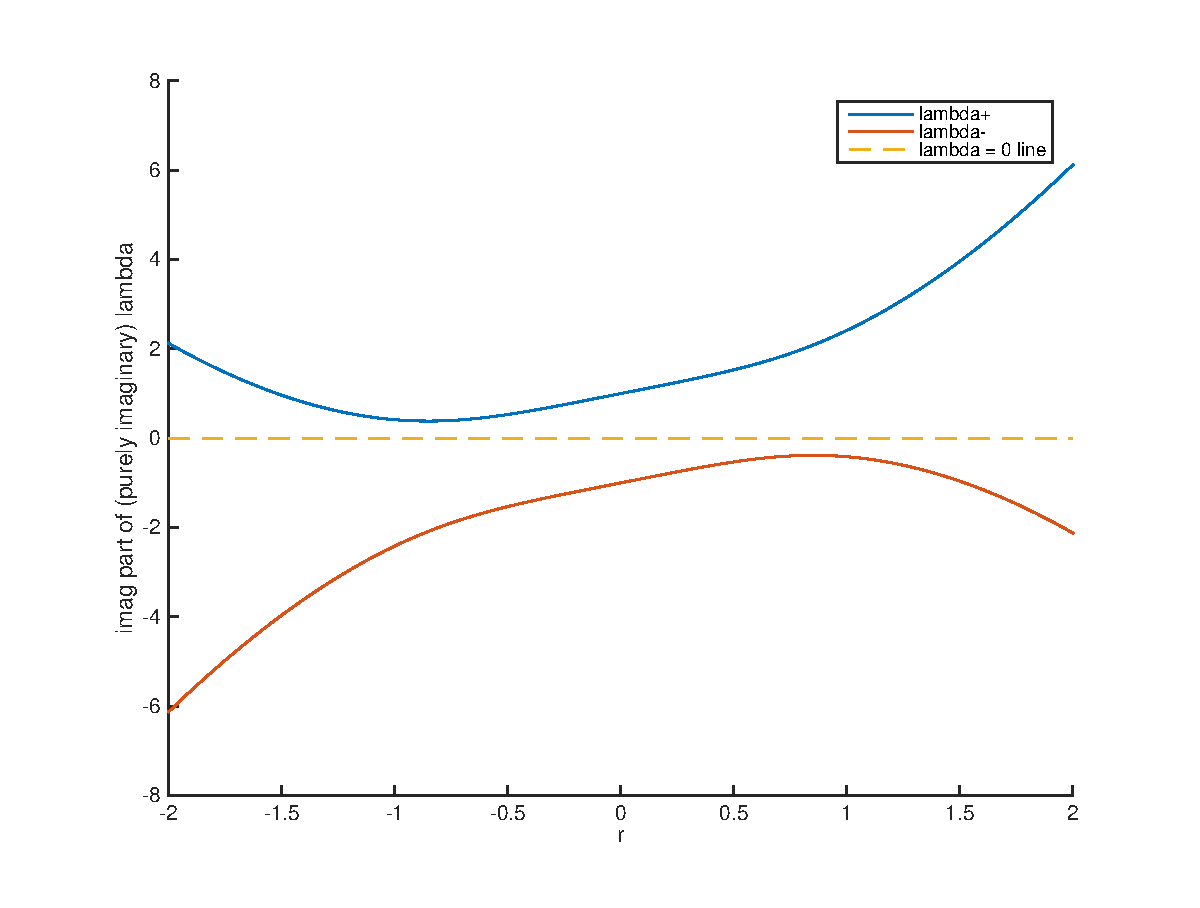
\includegraphics[width=10cm]{essspec1.eps}
\label{fig:essspec1}
\caption{Imaginary part of the purely imaginary essential spectrum for $c = 1$.}
\end{figure}

The equation for $\lambda(r)$ is of the form $\lambda_\pm(r) = k r \pm f(r^2)$. Since

\begin{align*}
\lambda_-(-r) = -kr - f((-r)^2) = -(kr + f(r^2)) = -\lambda_+(r)
\end{align*} 

and we take $r \in \R$, it suffices to look at $\lambda_+(r)$. Using Mathematica, we find

\begin{align*}
\lambda_+'(r) = c+\frac{2 r^3}{\sqrt{r^4+1}}
\end{align*}

Solving $\lambda_+'(r) = 0$ involves solving the 6th order polynomial

\[
4 r^6 - c^2 r^4 + c^2 = 0
\]

Mathematica will actually do it (!), but it is an epic mess. So we will look at it numerically using Matlab. The next plot shows the minimum value of $\lambda_+(r)$ as a function of $c$. Note that for $c = 0$ this minimum is clearly $0$, and for $c = \sqrt{2}$ it is not hard to show that this minimum is actually 0 (hence no essential spectrum gap.) $c = \sqrt{2}$ is the bifurcation point mentioned above, so this is consistent.

\begin{figure}[H]
\centering
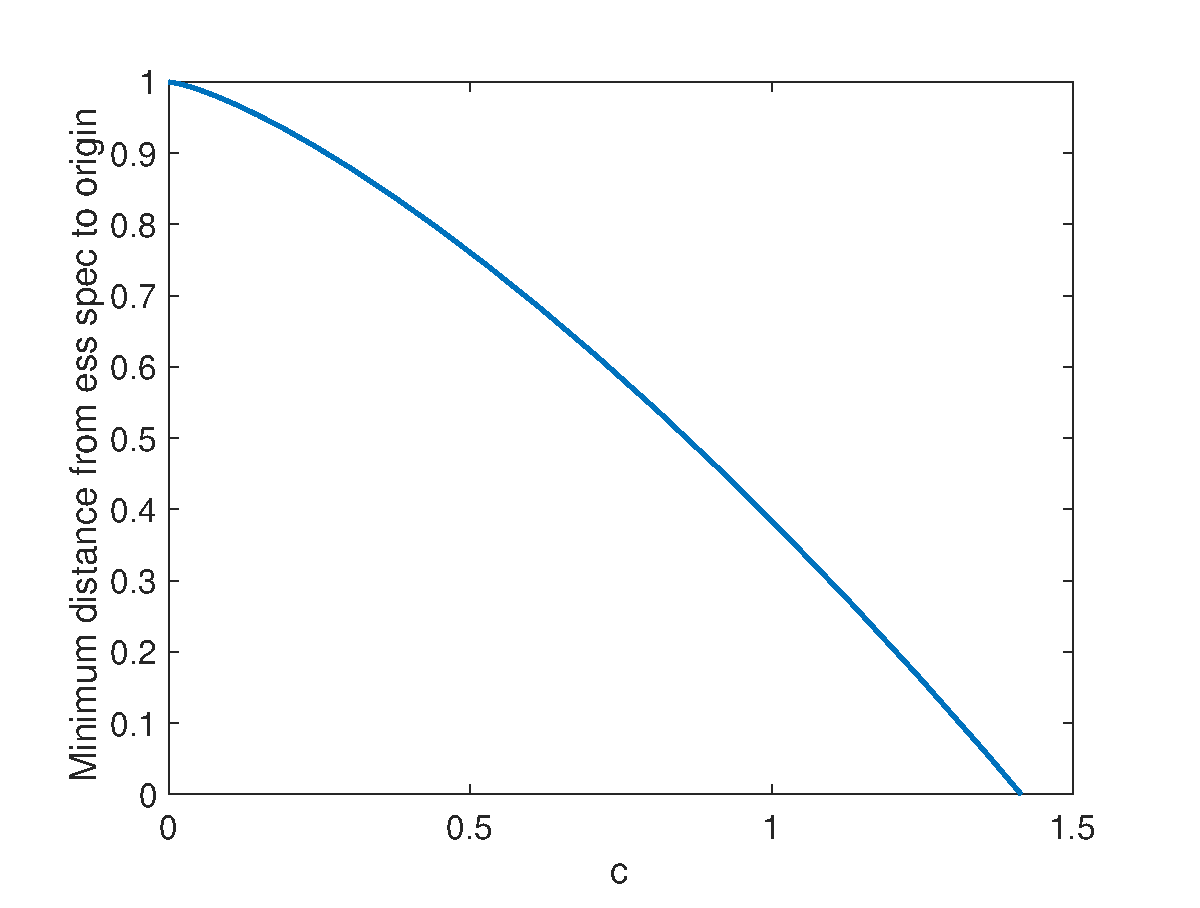
\includegraphics[width=10cm]{minlambdaplus.eps}
\label{fig:essspec1}
\caption{Imaginary part of the purely imaginary essential spectrum for $c = 1$.}
\end{figure}

Note that this minimum decreases strictly as $c$ increases, so the essential spectrum gap narrows (to 0) as $c$ increases from 0 to $\sqrt{2}$.\\

We could probably do better, i.e. approximate or get an exact formula (likely a nasty one) for this curve, but this is good enough for now.\\

When we compute the spectrum numerically with Matlab (details on how we do this are below), we see this essential spectrum gap around the origin. For $c = 1.2$, Matlab predicts that the essential spectrum gap is $[-0.2061, 0.2061]$. Here are plots of the computed spectrum from Matlab of the linearization about the single pulse solution. These show this essential spectrum gap. The eigenvalues at 0 are from translation invariance, which are discussed below.

\begin{figure}[H]
\centering
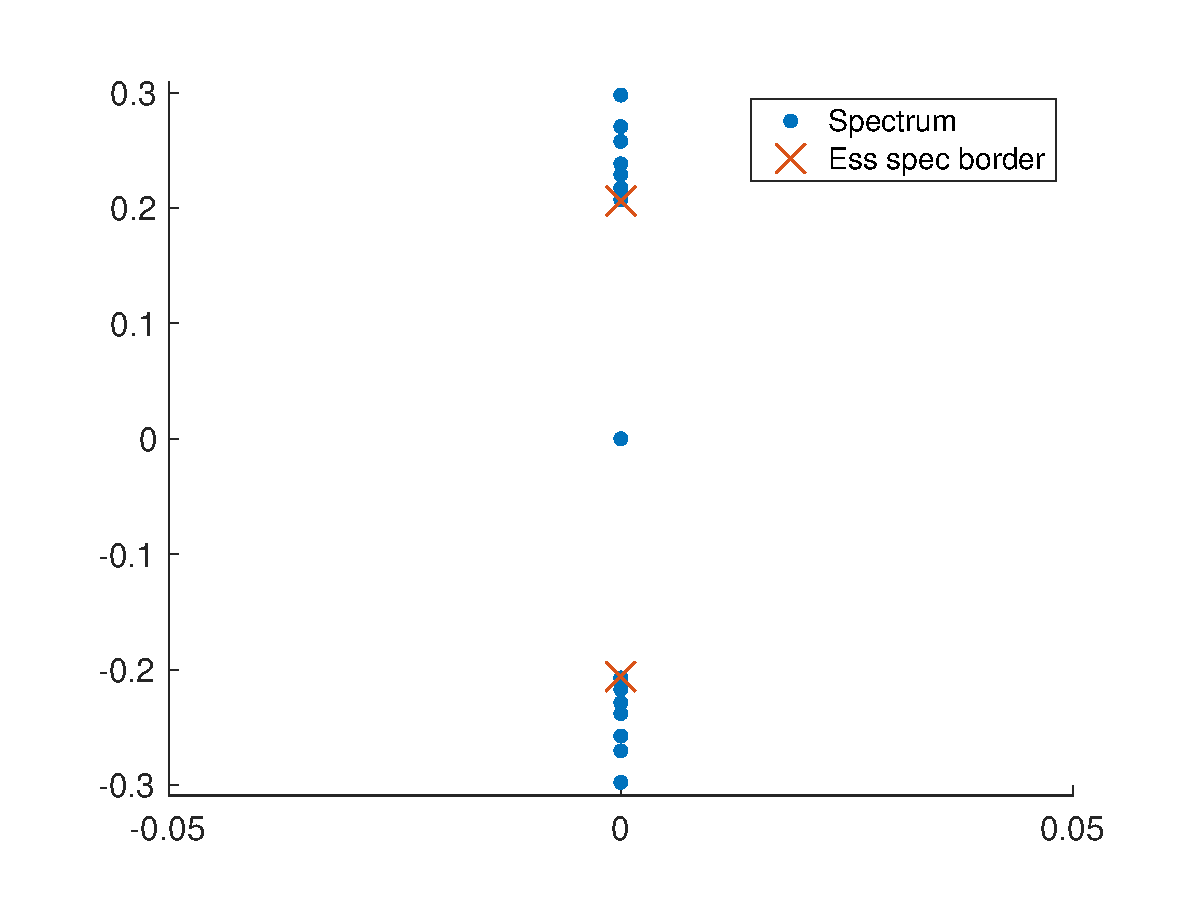
\includegraphics[width=8cm]{essspecboundsF256.eps}
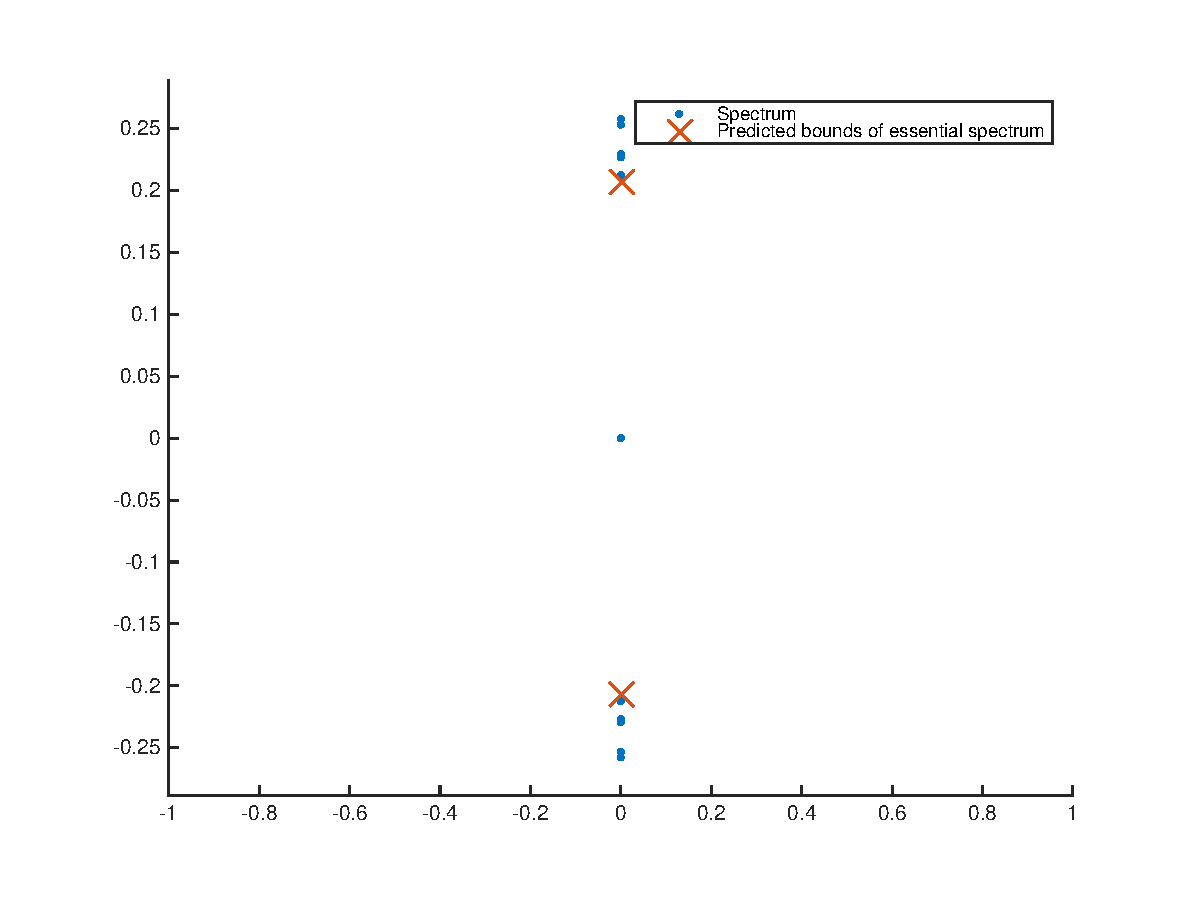
\includegraphics[width=8cm]{essspecboundsFD256.eps}
\caption{Essential spectrum gap for $c = 1.2$. Fourier spectral methods, $N = 256$ (left), finite difference methods, $N = 256$ (right)}
\end{figure}

Now that have looked at the essential spectrum, we can move on the point spectrum. There are only a few things we can say at this point.\\

If $\lambda = 0$, the eigenvalue problem reduces to

\begin{equation*}
A_0 v = (\partial_x^4 + c^2 \partial_x^2 + e^{u_*})v = 0
\end{equation*}

If we take $v = \partial_x u_*$, then 
\begin{align*}
A_0 \partial_x u_* &= 
(\partial_x^4 + c^2 \partial_x^2 + e^{u_*})\partial_x u_* \\
&= \partial_x[(u_*)_{xxxx} + c^2 (u_*)_{xx} + e^{u_*}] \\
&= \partial_x(1) \\
&= 0
\end{align*}

where we use the fact that $u_*$ is an equilibrium solution, thus must satisfy \eqref{eqODE}. Thus 0 is an eigenvalue of \eqref{evp} with corresponding eigenfunction $\partial_x u_*$.\\

When we solve for the eigenvalues numerically (again, details below), we get eigenvalues (close to) 0, but both eigenfunctions look like the derivative of $u_*$. In this case, I don't think we can have a generalized kernel function since the operator $A_0$ is self-adjoint, so by the Fredholm alternative we cannot have a function $v$ such that $A_0 v = \partial_x u_*$. (Otherwise $\partial_x u_*$ would be perpendicular to the kernel of $A_0^* = A_0$, which is impossible.)\\

Best guess is that we get two eigenvalues at 0 from the quadratic solver because of how it works.\\

We also want to look at the derivative with respect to the speed $c$, since it often shows up in these types of problems. Taking the derivative of \eqref{eqODE} with respect to $c$, we get

\begin{align*}
0 &= u_{xxxxc} + 2 c u_{xx} + c^2 u_{xxc} + e^{u} u_c \\
&= 2 c u_{xx} + (\partial_x^4 + c^2 \partial_x^2 + e^{u})u_c
\end{align*}

At an equilibrium solution $u_*$, we rearrange this to get

\begin{align*}
(\partial_x^4 + c^2 \partial_x^2 + e^{u^*})u^*_c &= -2 c u^*_{xx}
\end{align*}

In other words, we have

\begin{equation}\label{uc}
A_0 \partial_c u^* = -2 c u^*_{xx}
\end{equation}

This will be useful later.

\subsection{Numerics, Construction of Solutions}

The big issue here is that stationary solutions to \eqref{eqODE} are hard to come by. Nonetheless, we have figured out a way to compute these numerically, although it is a bit dicey. Our method is a variant of the mountain pass and string methods, and essentially combines Chen97 and Chamard10.

\begin{enumerate}
	\item The energy functional $I \in C^1(H^2, \R)$ is given by
	\begin{equation}
	I(z) = \frac{1}{2} \int_\R (|z''|^2 - c^2 |z'|^2)dx 
	+ \int_\R (e^z - z - 1) dx
	\end{equation}
	where $z$ is a function of $x$. For the numerical method, we truncate the domain to $[-L, L]$ for $L$ large.
	\item To do the mountain pass method, we need to find
	\begin{enumerate}
		\item A function $e_1 \in H^2$ which is a local minimum of $I$. From Lemma 2.4 in Chen97, $e_1 = 0$ satisfies this.
		\item A function $e_2 \in H^2$ for which $I(e_2) < I(e^1) = I(0) = 0$. We can use Lemma 2.5 in Chen97 to find such an $e_2$. 
	\end{enumerate} 
	The solution we want, by the Mountain Pass Lemma, is the infimum of the maxima of $I$ along all paths joining $e_1$ and $e_2$.
	\item Choose a discretization scheme. Following Chen97, we use the finite difference method.
	\item We then use the String Method from Chamard10.
	\begin{enumerate}
		\item Join $e_1$ and $e_2$ by a piecewise linear path $U(t) = t e_1 + (1-t) e_2 = (1-t)e_2$. Choose a discrete set of values for $t$ which are evenly spaced, i.e. the $N+1$ values $t = [0, 1/N, 2/N, ..., 1]$ for some reasonably sized $N$. We ended up using $N = 10$, which worked fine.
		\item Reparameterize the path to get points more-or-less equidistantly distributed in the $H^1$ norm.
		\item Evaluate the steepest decent direction $v(t_i)$ for all points $U(t_i)$ along the path. The steepest descent direction is computed as in section 3 of Chen97.
		\item For constrained maximal step size $h_M$, perform gradient descent on all points on the path $U(t_i)$ in the direction of $v(t_i)$.
		\item Go back to the reparameterization step, and repeat all this a bunch of times. Theoretically there is a termination condition, but we don't actually need to worry about that since we will be using Matlab's \texttt{fsolve}.
	\end{enumerate}
	\item After doing this a bunch of times, take the element of the path for which $I(U(t_i))$ is maximum. Or take one close to the maximum. Use this as an initial guess for Matlab's \texttt{fsolve}. This should converge to the solution we are looking for.
\end{enumerate}

Here are plots of the stationary solution $u(x)$ found using this method for $c = 1.354$ and $c = 1.40$. Compare these to figure 3 on p. 347 of Chen97. Note that by the substitution we performed, the baseline in our plots is at 0 as opposed to 1 in Chen97.

\begin{figure}[H]
\centering
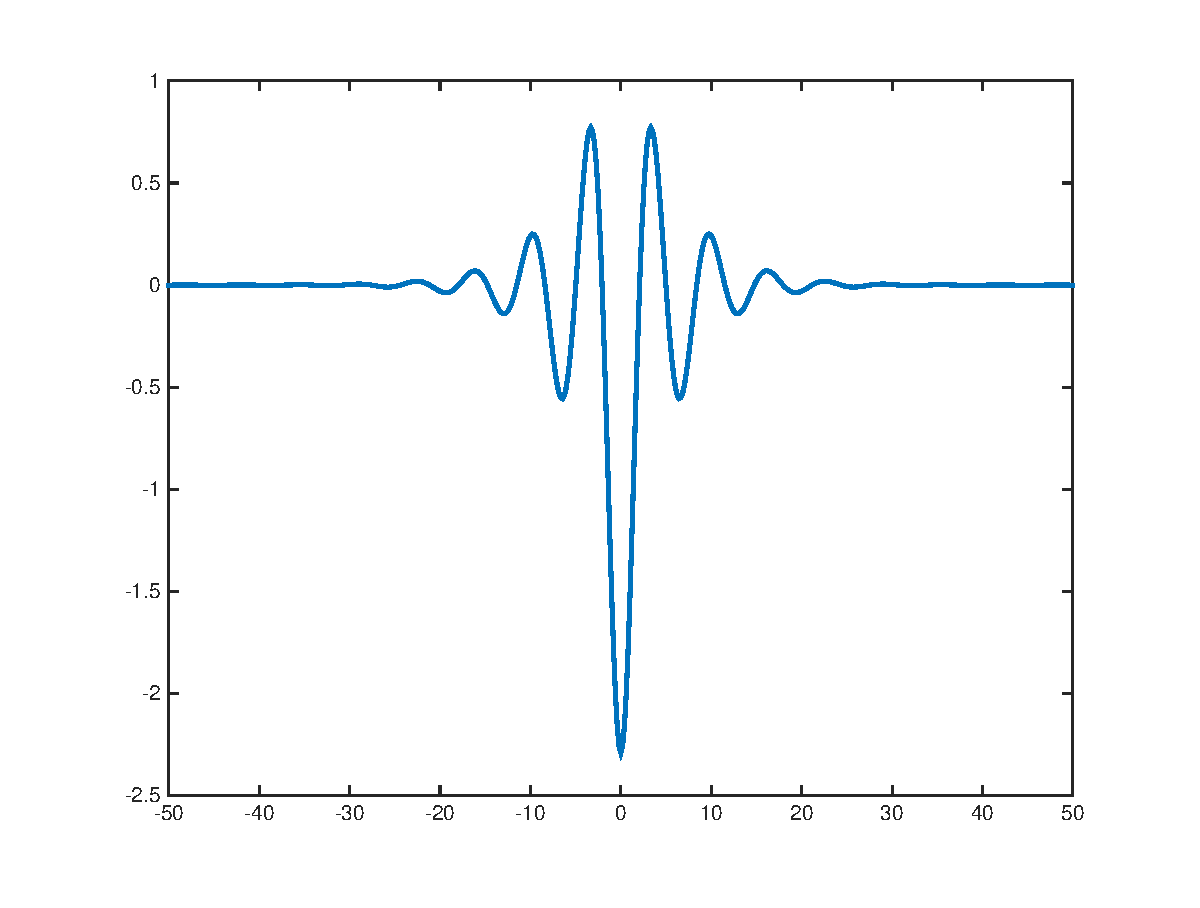
\includegraphics[width=8cm]{single1354.eps}
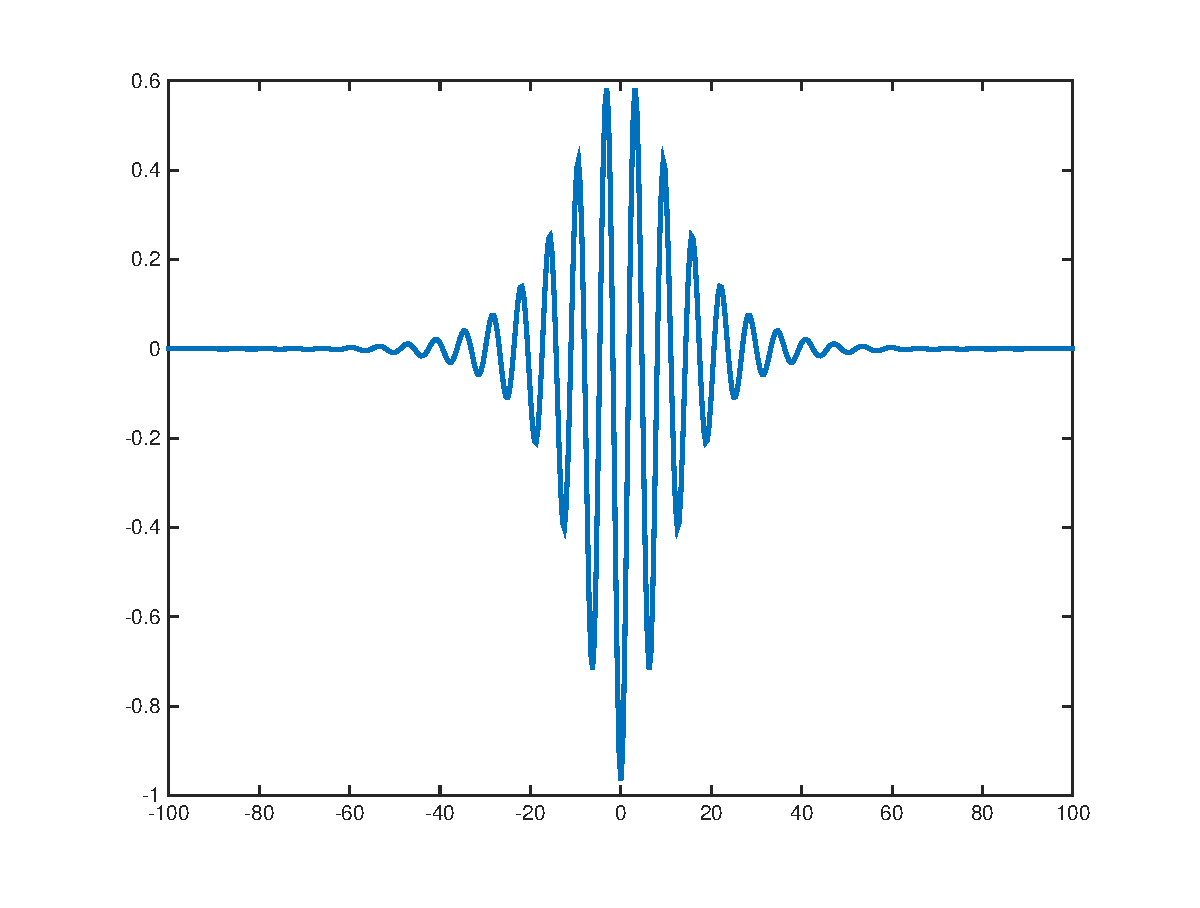
\includegraphics[width=8cm]{single14.eps}
\label{fig:single1}
\caption{Stationary traveling wave solutions to \eqref{eqODE}. $c = 1.354$ (left) and $c = 1.40$ (right).}
\end{figure}

We also compute solutions for other values of $c$.

\begin{figure}[H]
\centering
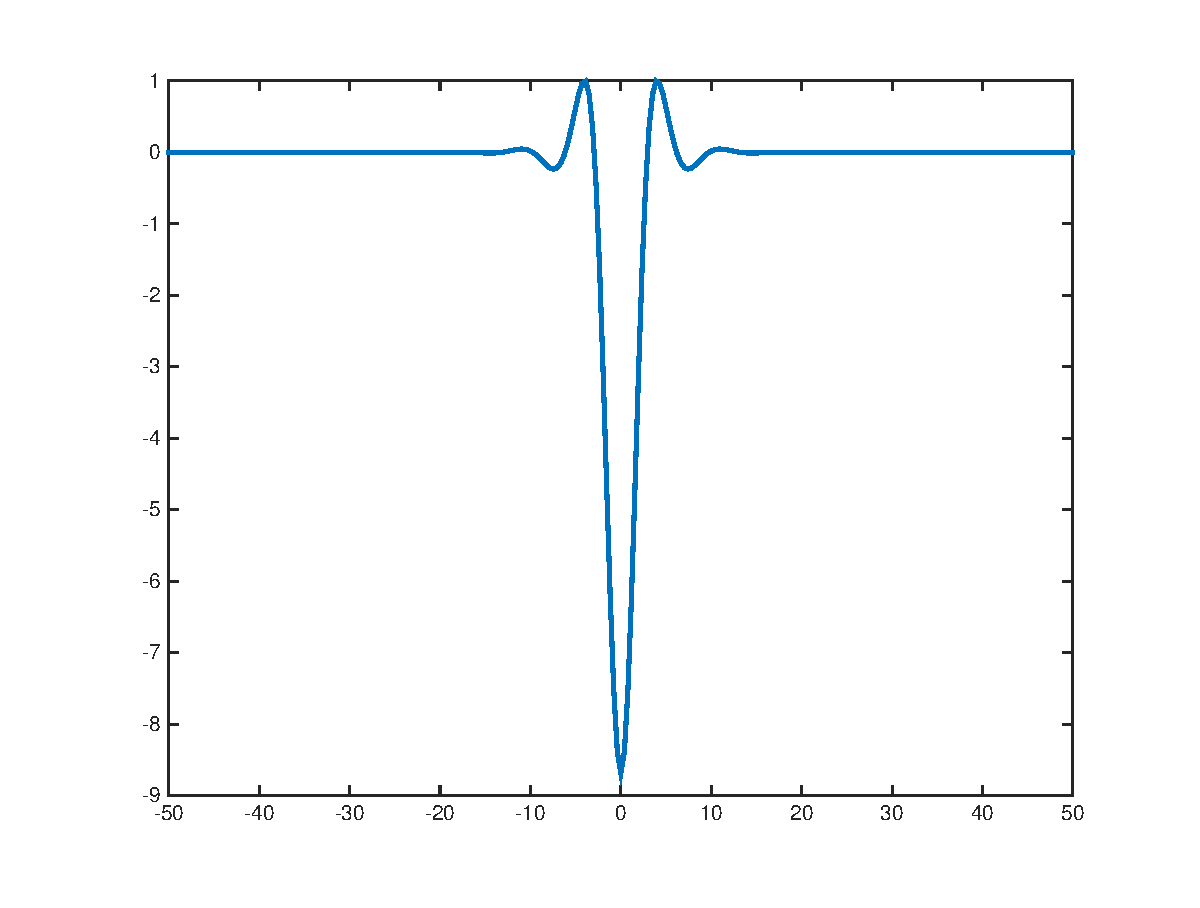
\includegraphics[width=8cm]{single11.eps}
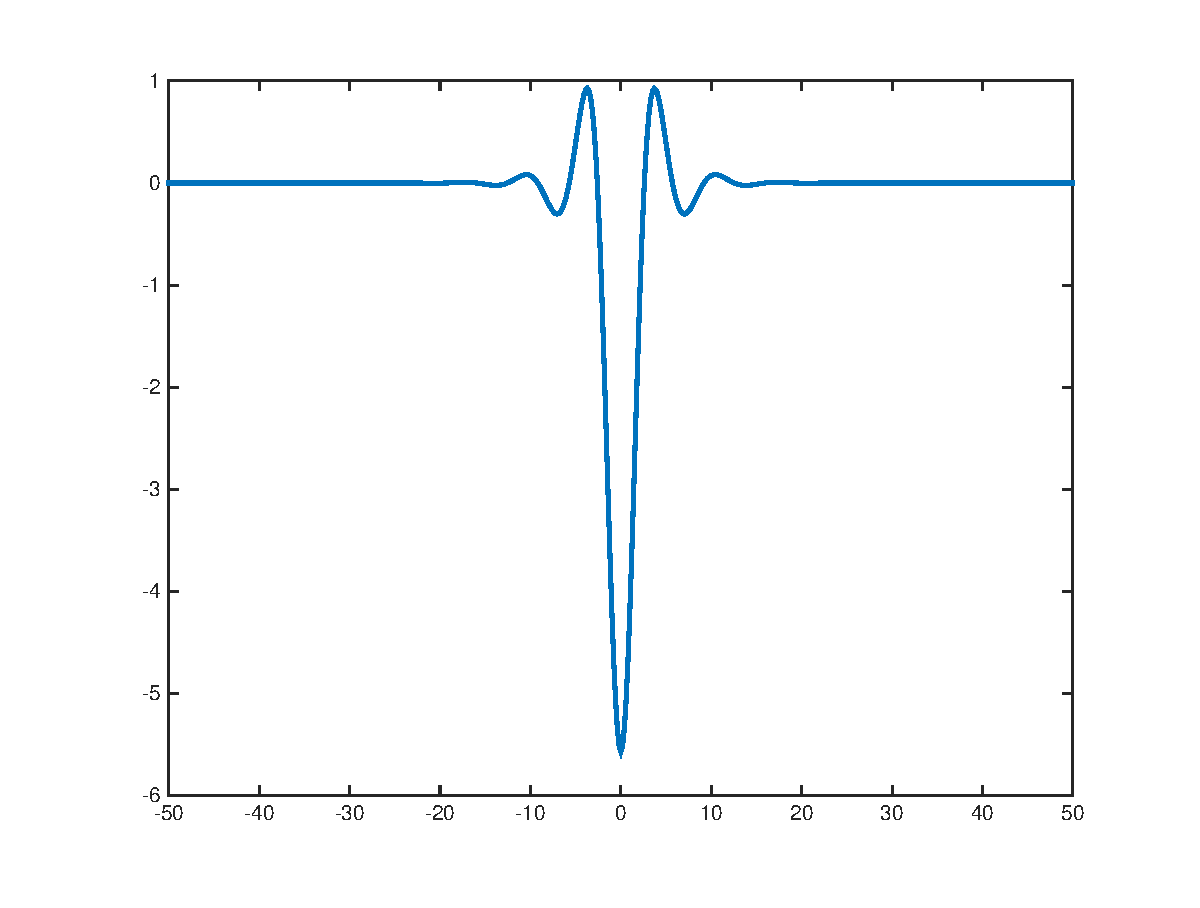
\includegraphics[width=8cm]{single12.eps}
\label{fig:single2}
\caption{Stationary traveling wave solutions to \eqref{eqODE}. $c = 1.1$ (left) and $c = 1.2$ (right).}
\end{figure}

Let $\nu = \pm \alpha \pm i \beta$ be the eigenvalues of the linearization about the zero solution. Then we can show numerically that the tail decays exponentially with rate (approximately) $\alpha$, and the period of the tail oscillations is (approximately) $2 \pi / \beta$. This is what we expect. \\

As in the other cases, we expect that we can join the tails to form double pulses every quarter period, i.e. every $\pi / 2 \beta$. Using the same method as we always use, together with Matlab's \texttt{fsolve}, here are the first four double pulses for $c = 1.2$.

\begin{figure}[H]
\centering
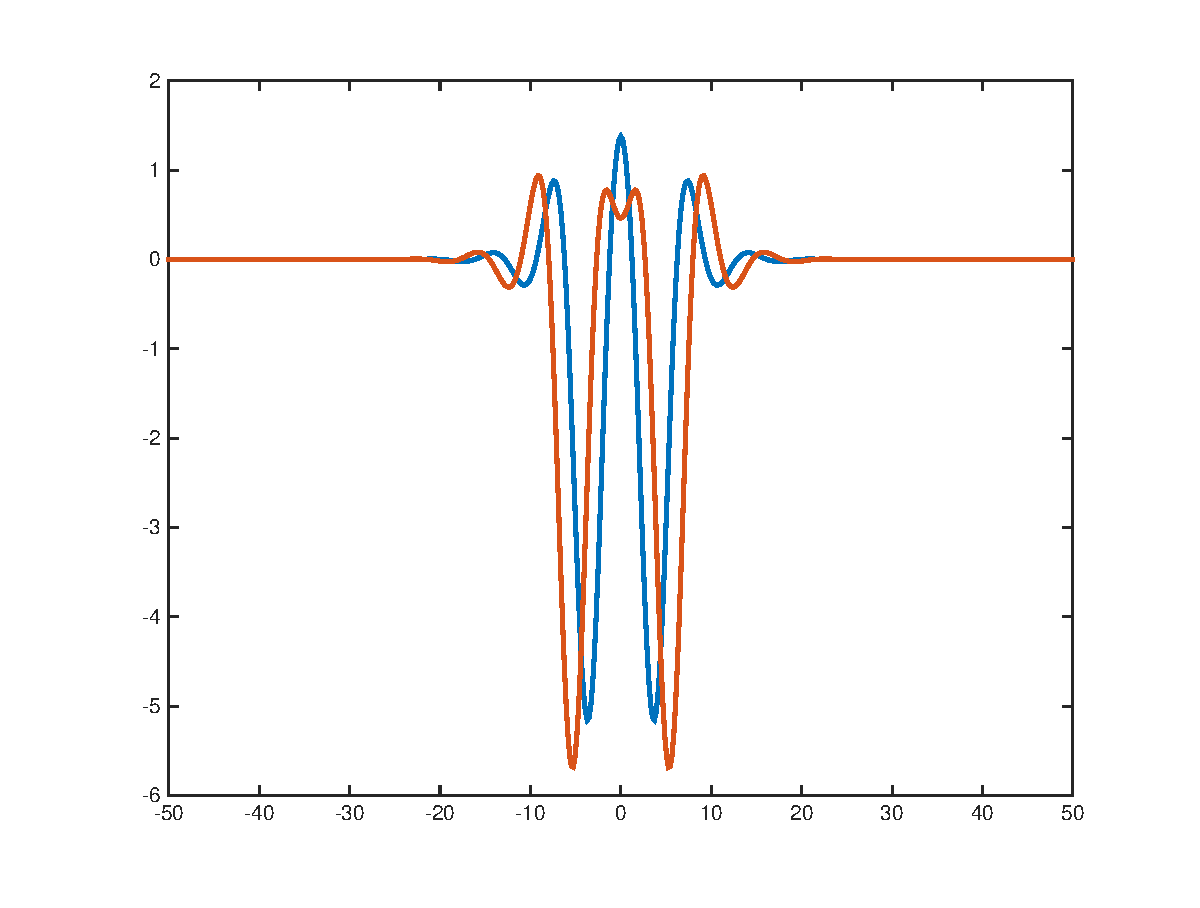
\includegraphics[width=8cm]{double12_12.eps}
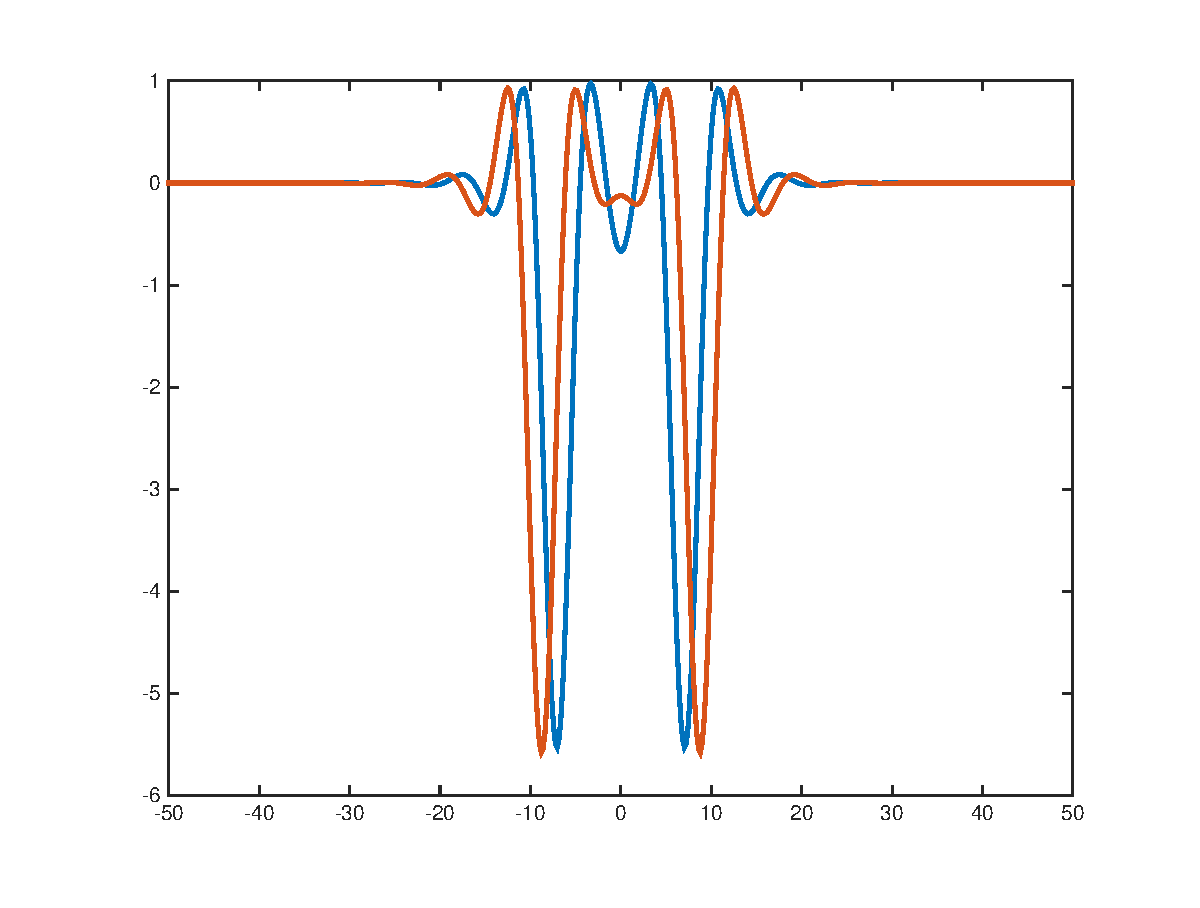
\includegraphics[width=8cm]{double12_34.eps}
% \caption{Double pulse traveling wave solutions to \eqref{eqODE} for $c = 1.2$. Double pulses 1 and 2 (left). Double pulses 3 and 4 (right).
\end{figure}

We can obtain periodic versions of all of these by interpolating the finite difference solutions onto the appropriate periodic grid, writing the operators using Fourier spectral matrices, and using \texttt{fsolve}. This is not shown.\\

\subsection{Numerics, Eigenvalue Computation}

It turns out that Matlab has a built-in polynomial eigenvalue solver, \texttt{polyeig}. However, I decided to use the quadratic eigenvalue solver \texttt{quadeig} by Chris Munro, Sven Hammarling and Francoise Tisseu (2013) because they say it's better. It probably makes very little difference.\\

Since this is going to look a lot like things I have already done (i.e. KdV5), I will not show all the plots. First, we look at $c = 1.2$.\\

For the first double pulse, here is the spectrum (zoomed near the origin) and a plot of the eigenfunctions corresponding to the small interaction eigenvalues. Note there is a pair of real interaction eigenvalues.

\begin{figure}[H]
\centering
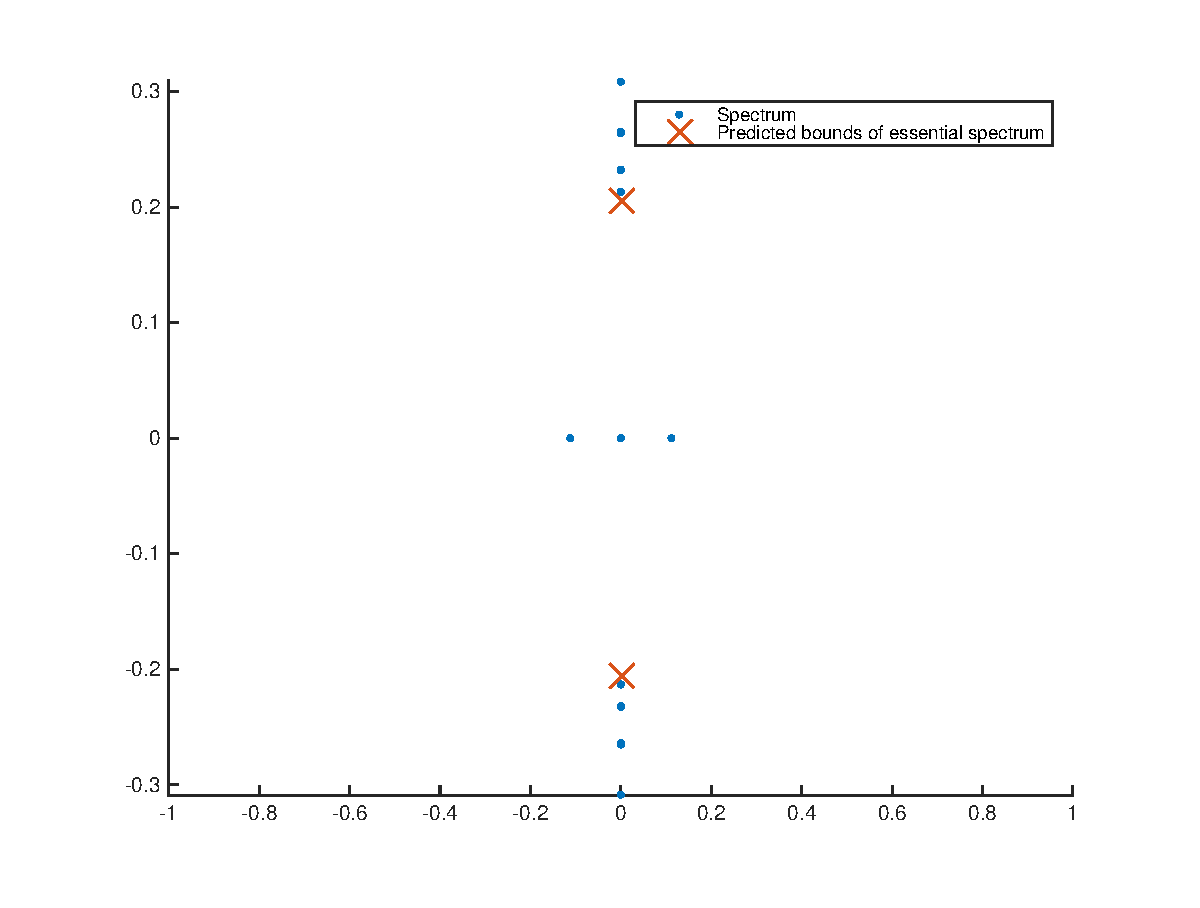
\includegraphics[width=8cm]{spec12_double1.eps}
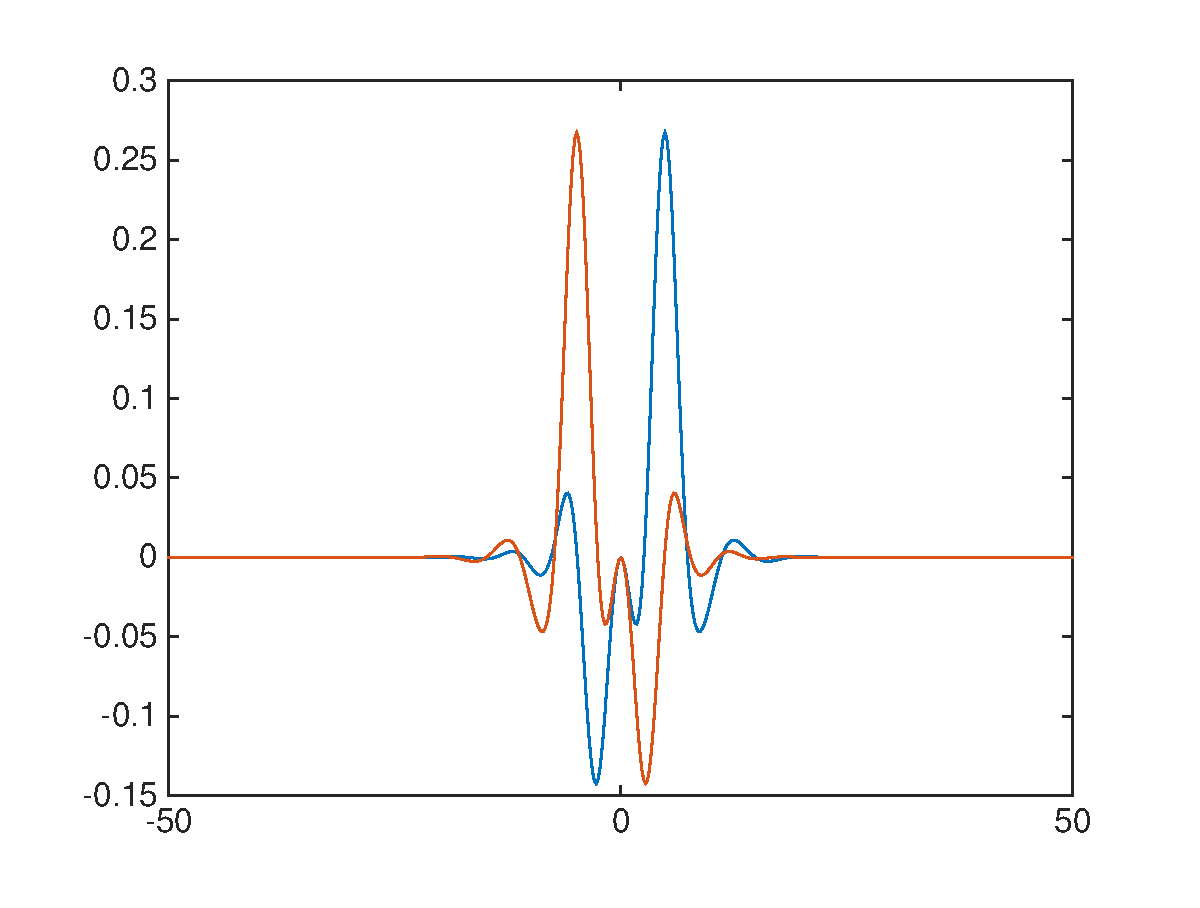
\includegraphics[width=8cm]{evecs12_double1.eps}
\caption{Linearization about Double Pulse 1. Spectrum (left) and interaction eigenfunctions (right). Finite difference methods, $N = 512$, $c = 1.2$.}
\end{figure}

Next we look at the second double pulse. Note that this time we have a pair of purely imaginary (to leading order, there is a small real part of order like 1e-10 just as with KdV5) eigenvalues. The plot below is only the real part of the eigenfunctions. It is easy to locate the interaction eigenvalues in this case, since we have bounds on the essential spectrum. The interaction eigenvalues lie inside the essential spectrum gap.

\begin{figure}[H]
\centering
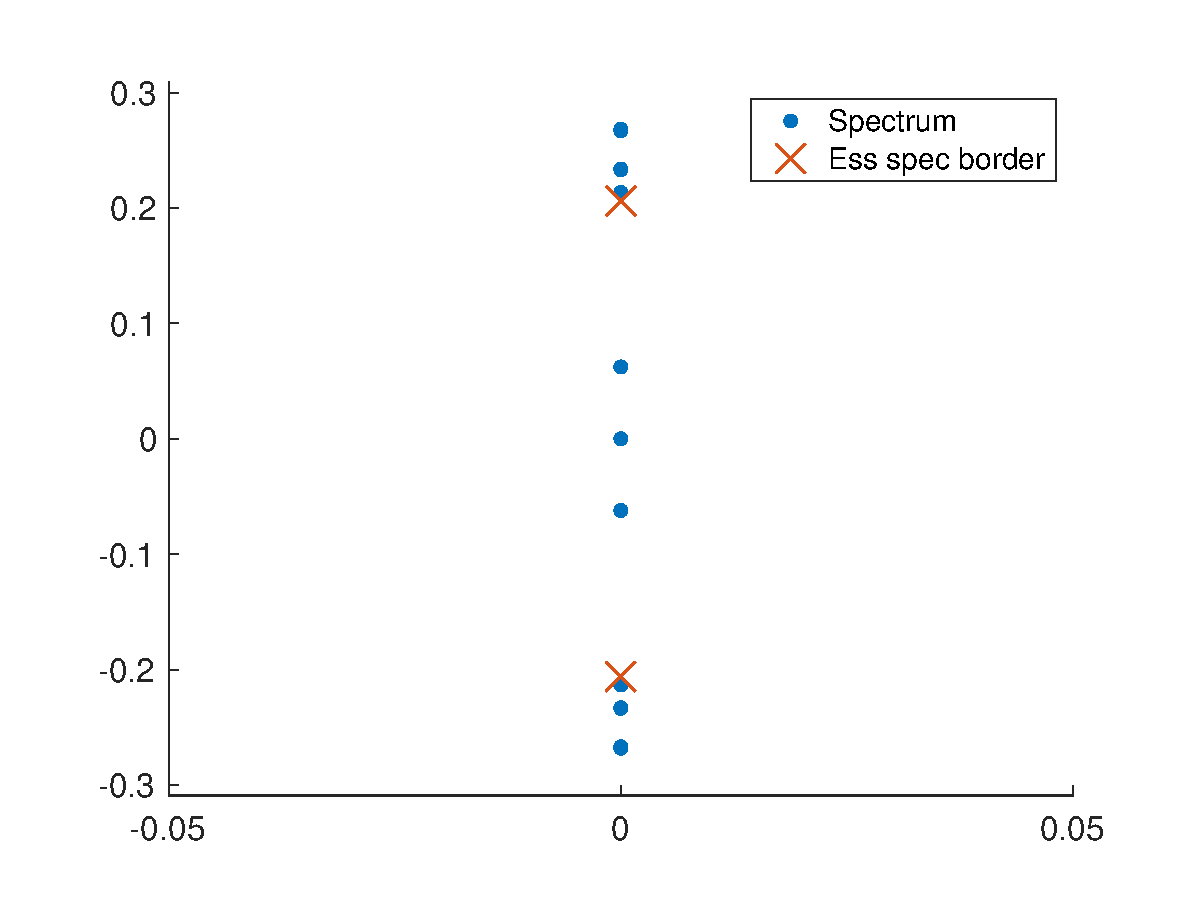
\includegraphics[width=8cm]{spec12_double2.eps}
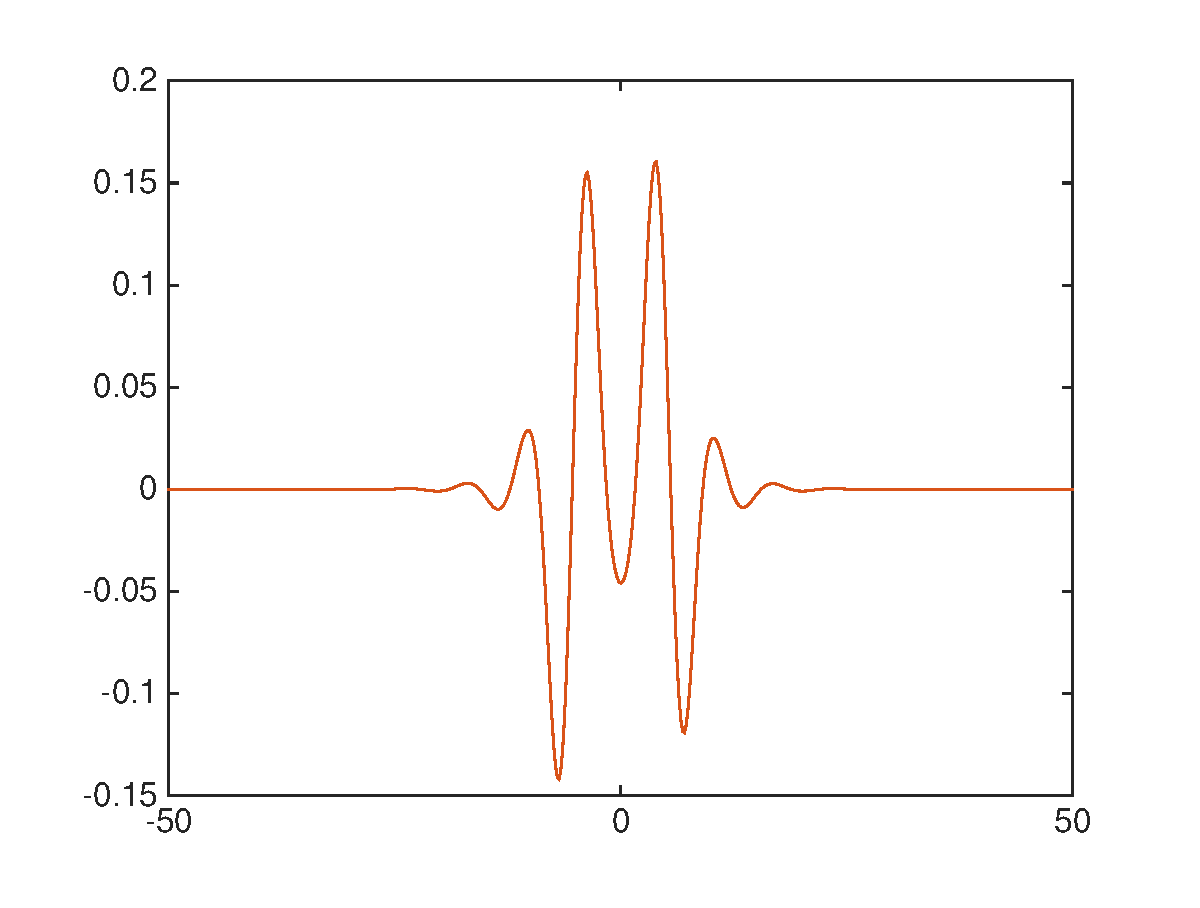
\includegraphics[width=8cm]{evecs12_double2real.eps}
\caption{Linearization about Double Pulse 2. Spectrum (left) and real part of interaction eigenfunctions (right). Finite difference methods, $N = 512$, $c = 1.2$.}
\end{figure}

The same pattern repeats (alternating real and purely imaginary interaction eigenvalues) as we go to higher double pulses.\\

We can also construct multipulses. For example, here is a triple pulse for $c = 1.2$ using the same pulse distance as double pulse 2. We get the expected two pairs of purely imaginary eigenvalues.

\begin{figure}[H]
\centering
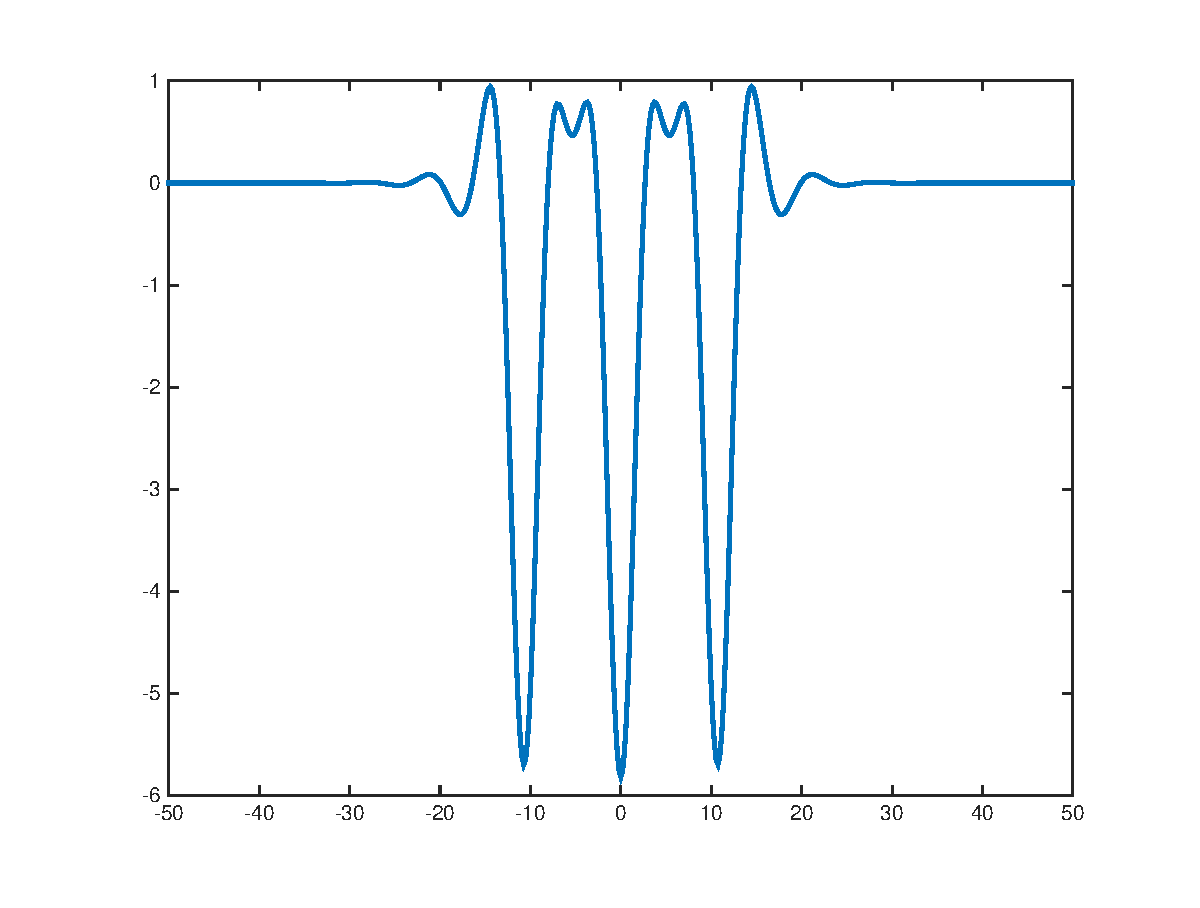
\includegraphics[width=8cm]{triple12_2.eps}
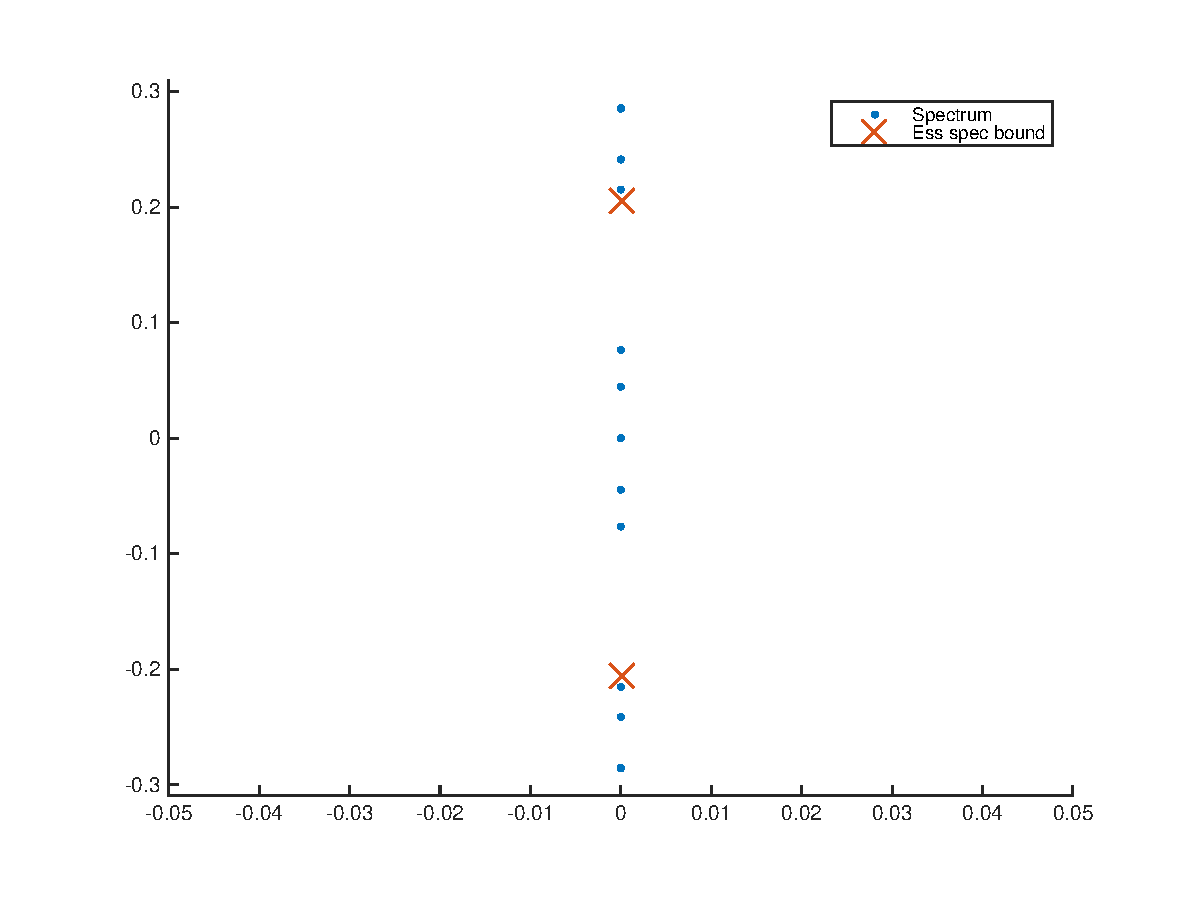
\includegraphics[width=8cm]{spec12_triple2.eps}
\caption{Triple pulse 2,2 (left). Spectrum of linearization about triple pulse 2,2 (right). Finite difference methods, $N = 512$, $c = 1.2$.}
\end{figure}

For other values of $c$, the odd-numbered double pulses have the same eigenvalue pattern, so we will focus on the even-numbered double pulses. Let's look at $c = 1.354$ (this value was used in Chen97). For Double Pulse 2, we now have a quartet of interaction eigenvalues. Their imaginary part now lies \emph{outside} the essential spectrum gap. This suggests that a Krein collision has occurred, where the interaction eigenvalues collide with the smallest essential spectrum eigenvalue and then form a quartet.

\begin{figure}[H]
\centering
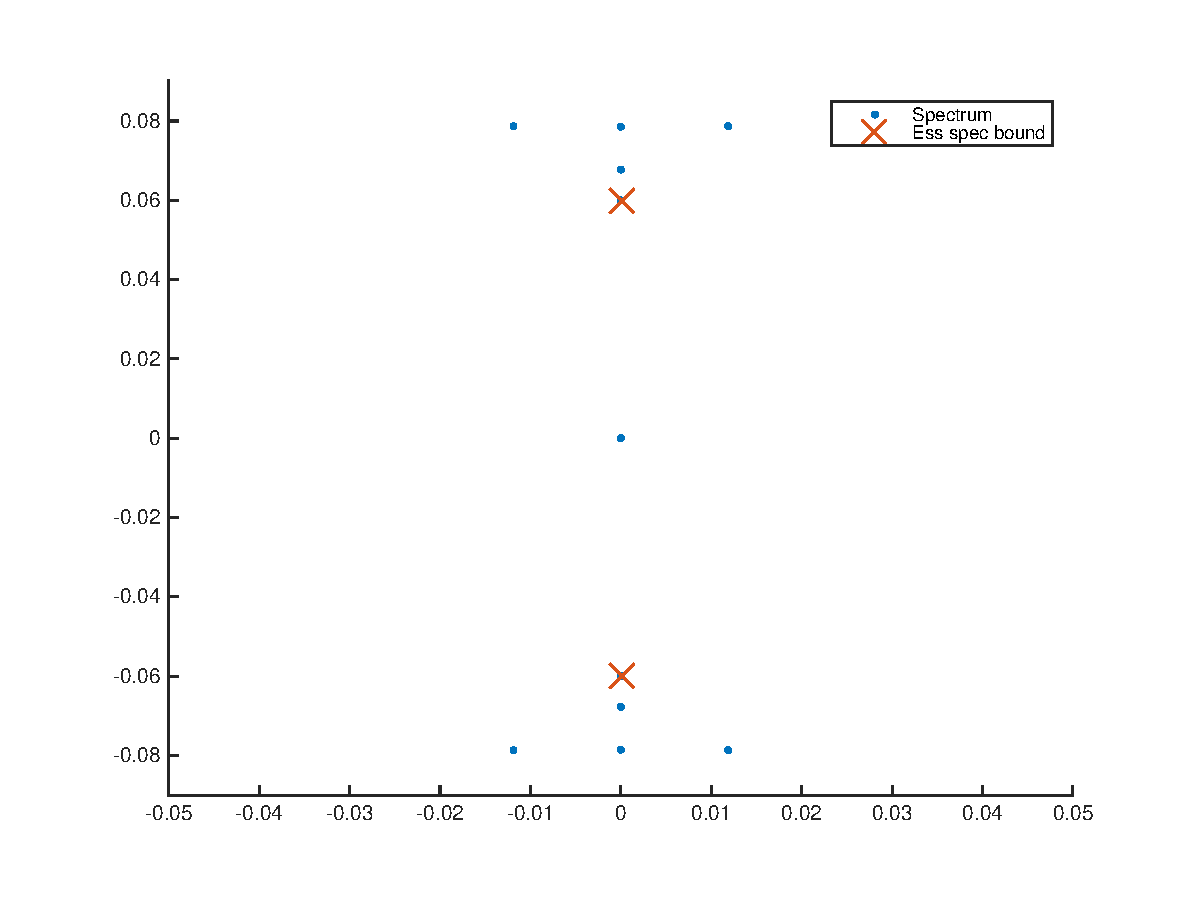
\includegraphics[width=8cm]{spec1354_double2.eps}
\caption{Linearization about Double Pulse 2. Spectrum showing Krein quartet. Finite difference methods, $N = 512$, $c = 1.354$.}
\end{figure}


The next two plots show that the Krein collision occurs between $c = 1.322$ (before collision) and $c = 1.323$ (after collision).

\begin{figure}[H]
\centering
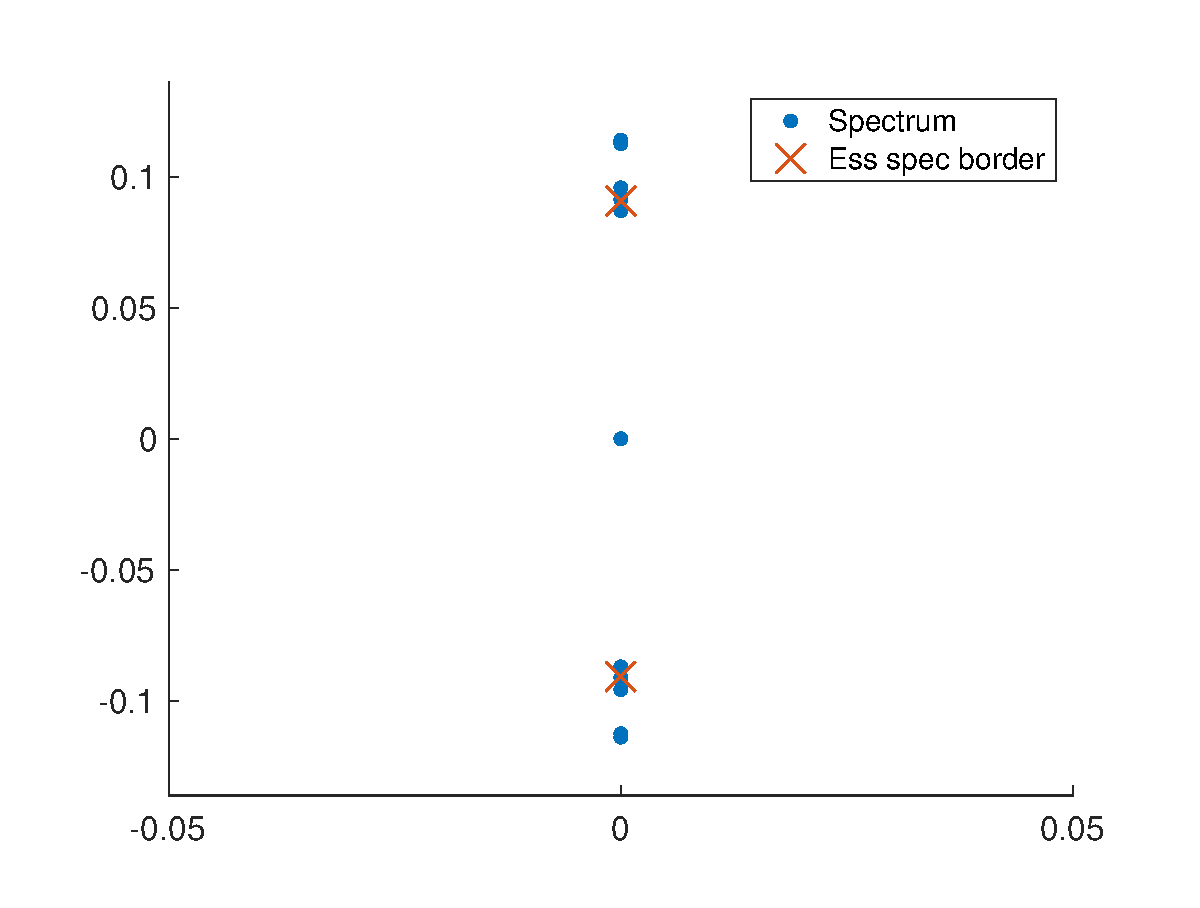
\includegraphics[width=8cm]{spec1322_double2.eps}
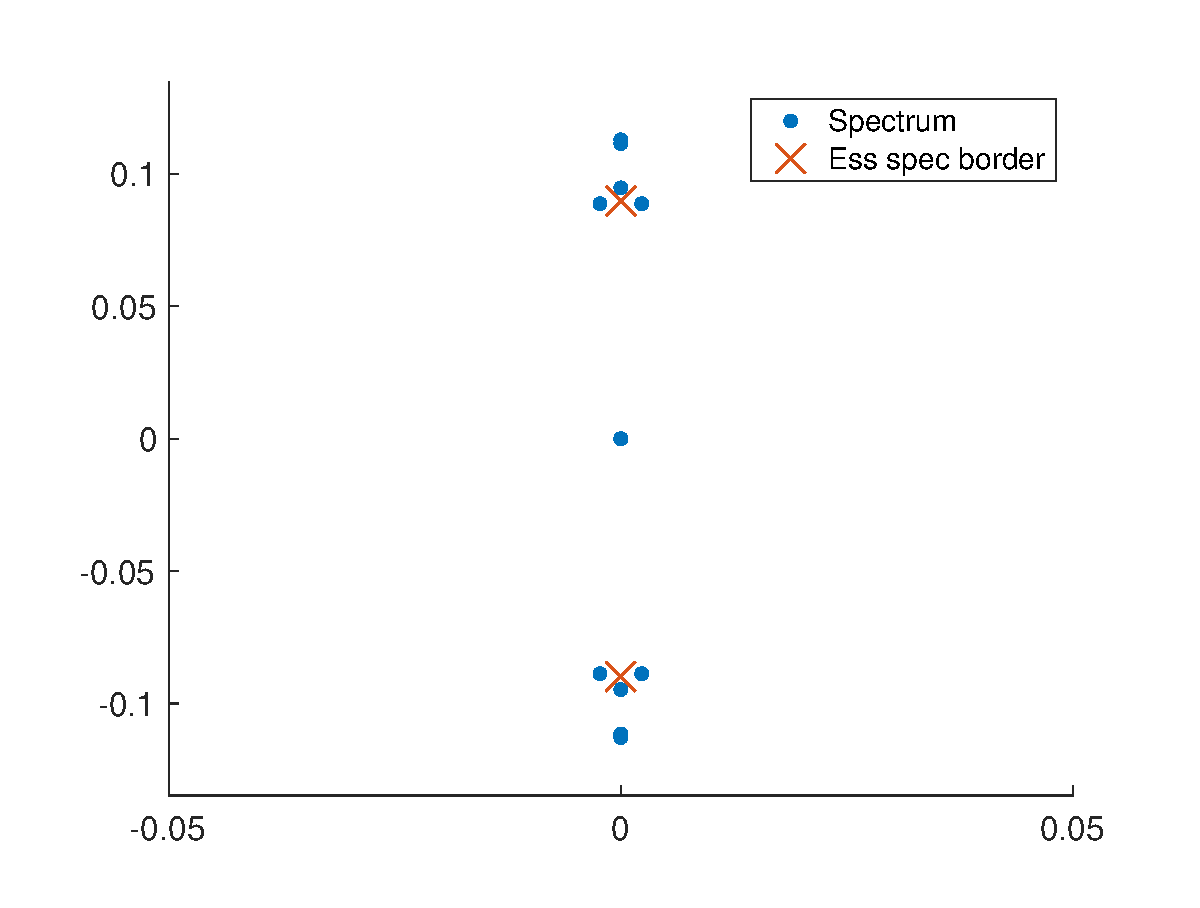
\includegraphics[width=8cm]{spec1323_double2.eps}
\caption{Linearization about Double Pulse 2. Spectrum before Krein collision ($c = 1.322$, left) and after Krein collision ($c = 1.323$, right). Finite difference methods, $N = 512$}
\end{figure}

\subsection{Lin's Method (part 1)}

In this section, we look at the eigenvalues of $A_0$, i.e. look at the eigenvalue problem

\[
A_0 v = \lambda v
\]

We expect this to be similar to SanStrut, since it's more-or-less the same thing but with a different nonlinearity. Using Matlab's \texttt{eig}, we can show that for the operator $A_0$ linearized about an $n-pulse$

\begin{enumerate}
	\item The essential spectrum is $[a, \infty)$ for some $a > 0$
	\item $n$ small eigenvalues near 0, one of which is actually at 0 (1D kernel)
	\item There are $n$ negative eigenvalues clustered near the negative eigenvalue of $A_0$ for the single pulse.
\end{enumerate}

We can verify this analytically.\\

In system-form, the operator $A_0$ is given by

\begin{equation}
A_0(\lambda; u_*) = \begin{pmatrix}
0 & 1 & 0 & 0 \\
0 & 0 & 1 & 0 \\
0 & 0 & 0 & 1 \\
\lambda - e^{u_*} & 0 & -c^2 & 0 
\end{pmatrix}
\end{equation}

where $u^*$ is an equilibrium solution. The essential spectrum only depends on the asymptotic matrix, so since all solutions $u^*(x)$ we will care about are decay exponentially to 0 at both ends, we only have to look at the asymptotic matrix

\begin{equation}
A_0(0) = \begin{pmatrix}
0 & 1 & 0 & 0 \\
0 & 0 & 1 & 0 \\
0 & 0 & 0 & 1 \\
\lambda - 1 & 0 & -c^2 & 0 
\end{pmatrix}
\end{equation}

The characteristic polynomial of this is

\[
p(\nu) = c^2 \nu^2 - \lambda + \nu^4 + 1
\]

Plugging in $\nu = i r$, this becomes

\[
p(i r) = c^2 r^2 - \lambda + r^4 + 1 = 0
\]

Solving for $\lambda$ gives us

\[
\lambda = r^4 + c^2 r^2 + 1 = r^2(r^2 + c^2) + 1
\]

from which we see that the essential spectrum is $\lambda = [1, \infty)$.\\

Using Lin's method (from San98) we can compute the small eigenvalues to leading order. It is easy to see that $q'$ is an eigenfunction with eigenvalue 0. For convenience, assume we a have an $n$-pulse, but assume that all the pulse distances are the same, say $2L$. (Of course, mixed-distance multipulses exist, but we will ignore that for now.) The, by Theorem 2 in San98, there are $n$ small eigenvalues which are given (to leading order) by solving $\det(aA - M \lambda I) = 0$. $M$ is the Melnikov integral, which in this case is

\begin{equation}
M = \int_{-\infty}^\infty (q'(x))^2 dx
\end{equation}

$A$ is the matrix

\begin{equation}
A = \begin{pmatrix}
-1 & 1 \\
1  & -2 & 1 \\
   & 1  & -2 & 1 \\
   & & \vdots & \vdots \\
   & & & & & 1 & -1
\end{pmatrix}
\end{equation}

and $a = \langle \Psi(L), Q'(-L) \rangle$, as in San98. For a 2-pulse, this becomes

\begin{align*}
\det \begin{pmatrix}
-a - M \lambda & a \\
a & -a - M \lambda
\end{pmatrix} = 0
\end{align*}

which has solutions $\lambda = \{ 0, -2a/M \}$. This is easy to compute numerically, so let's see if this agrees with what we get if we use \texttt{eig} on $A_0$.

\begin{table}[H]
\begin{tabular}{llll}
Double Pulse & Eigenvalue from eig(A0) & Predicted eigenvalue (-2a/M) & Error  \\
1            & 0.1278                  & 0.1915                       & .5     \\
2            & -0.0278                 & -0.0254                      & 0.08   \\
3            & 0.0090                  & 0.0072                       & .20    \\
4            & -0.0024                 & -0.0025                      & 0.0417 \\
5            & 6.8497e-04              & 7.2475e-04                   & 0.0581
\end{tabular}
\caption{Calculated and predicted small eigenvalue of $A_0$ about Double Pulse 2. $c = 1.2$. Finite difference methods, $N = 1500$}.
\end{table}

Well, it's not great, but the error does decrease as $L$ increases, so it should be ok. For the triple pulse we have to solve

\begin{align*}
\det \begin{pmatrix}
-a - M \lambda & a & 0\\
a & -2a - M \lambda & a \\
0 & a & -a - M \lambda
\end{pmatrix} = 0
\end{align*}

which has solutions $\lambda = \{ 0, -a/M -3a/M \}$.\\

For $c = 1.2$ and triple pulse 2,2, we have small eigenvalues from \texttt{eig} of $\{ -0.0145, -0.0401 \}$. The formula above predicts eigenvalues of $( -0.0127, -0.0381 \}$. The errors here are $0.049$ and $0.124$, which are not terrible.\\

We don't really care about this, except to contrast to the quadratic eigenvalue problem.\\

Similarly, using a method similar to SanStrut, we can show that $A_0(q)$ has a single negative eigenvalue, and we can use Lin's method to show that $A_0(q_n)$ has a $n$ negative eigenvalues all of which are close to the single negative eigenvalue of $A_0(q)$.

\subsection{Krein Matrix}

\subsubsection{Background and Numerics}

Before we do that, we can look at the Krein matrix as means of computing eigenvalues in the case where they are (predicted to be) purely imaginary. The hope is that we can get theoretical results for the 2-pulse and nice numerics for the n-pulse.
\\

This is an application Todd Kapitula's unpublished paper Krein Matrix for Star-Even Operator Polynomials (2018). Here we look at the polynomial eigenvalue problem for the suspension bridge problem linearized about stationary solution $q$. This second degree eigenvalue problem is given by

\begin{equation}
p(\lambda)v = (A_0 + A_1 \lambda + A_2 \lambda^2 )v = 0
\end{equation}

where

\begin{align*}
A_0 &= \partial_x^4 + c^2 \partial_x^2 + e^{q} \\
A_1 &= - 2 c \partial_x \\
A_2 &= I 
\end{align*}

Note that $A_0$ and $A_2$ are Hermitian, and $A_1$ is skew-Hermitian.\\

The Krein matrix should work perfectly in this case, since we don't have to deal with invertibility of operators and since the essential spectrum is purely imaginary and bounded away from the origin.\\

We know from the discussion in the previous section what the spectrum/eigenvalues of $A_0$ looks like. Since $A_0$ is Hermitian, the spectrum of $A_0$ is real. We also note that if we take $\lambda = i z$, the quadratic operator $p(iz)$ is Hermitian.
\\

Let $S = \spn\{s_1, \dots, s_n \}$, where $s_i$ are the eigenfunctions of $A_0$ corresponding to the small eigenvalues $\{\nu_1, \dots, \nu_n$. (We found these in the previous section using Lin's method). WLOG, we take $\nu_1 = 0$ and $s_1 = q'$, since we know the kernel of $A_0$ is 1-dimensional, and we know what the kernel eigenfunction is. We also note that since $A_0$ is self-adjoint and the eigenvalues $\nu_i$ are distinct, the corresponding eigenfunctions $s_i$ are orthogonal.

With this setup, we can easily compute the Krein matrix using the top of p.4 in Kap2018. As long as as choose $c$ such that the Krein collision has not yet occurred, we get very accurate numerical results from this method, or at least they compare extremely well to the quadratic eigenvalue solver we are using. 

\begin{table}[H]
\begin{tabular}{lll}
Pulse & From \texttt{quadeig} & imag part (from Krein Matrix) \\
Double Pulse 2    & $\pm 0.0622i$ & 0.0622 \\
Triple Pulse 2,2  & $\pm 0.0446i, \pm 0.0764i$ & 0.0446, 0.0764 \\
Double Pulse 2    & $\pm 0.0176i$ & 0.0176 \\
\end{tabular}
\caption{Eigenvalues from quadratic eigenvalue problem, computed with \texttt{quadeig} and from the Krein matrix. $c = 1.2$, finite difference method, $N = 512$. }
\end{table}

So, basically, the Krein matrix nails it every time.\\

\subsubsection{Approxmation for Small Eigenvalues}

Now that we know we can use the Krein matrix, we should be able to use the approximation as in Section 5 of Kap2018 since these eigenvalues are small.\\

Recall that we are looking for purely imaginary eigenvalues, thus we take $\lambda = i z$, $z \in \R$. Then the operator $p(iz)$ is Hermitian, which implies that the Krein matrix is also Hermitian (p. 6 of Kap2018). By Lemma 5.6 in Kap2018, for small $|z|$ the Krein matrix is the $n \times n$ matrix

\begin{equation}
K_S(z) = \text{diag}(\nu_1, \dots, \nu_n) + \overline{z} K_1 - \overline{z}^2 \tilde{K}_2 + \mathcal{O}(|z|^3)
\end{equation}

where

\begin{equation}
(K_1)_{jk} = \langle s_j, i A_1 s_k \rangle
\end{equation}

and

\begin{equation}
(\tilde{K}_2)_{jk} = \langle s_j, (A_2 - A_1 P_{S^\perp} (P_{S^\perp} A_0 P_{S^\perp})^{-1} P_{S^\perp} A_1 ) s_k  \rangle
\end{equation}

Note that we omit the $z$ out front from Lemma 5.6, i.e. we use the form of the Krein matrix from p.4 rather than the form in Theorem 3.1. The key observation is that this is, to leading order, a matrix-valued quadratic polynomial in $z$.

Since the operator $A_1$ is skew-Hermitian, $i A_1$ is Hermitian, thus for $K_1$ we have

\begin{align*}
(K_1)_{jk} = \langle s_j, i A_1 s_k \rangle &= \langle i A_1 s_j, s_k \rangle \\
&= \overline{ \langle s_k, i A_1 s_j \rangle } \\
&= \overline{ (K_1)_{kj} }
\end{align*}

Thus, as expected, $K_1$ is a Hermitian matrix. In particular, this implies that the diagonal entries are real. Since $A_0$ and the eigenfunctions $s_i$ are real, $(K_1)_{ii} = \langle s_i, i A_1 s_i \rangle = \langle s_i, i A_1 s_i \rangle$ is purely imaginary, thus must be 0. We conclude that diagonal terms of $K_1$ are 0.\\

For the matrix $\tilde{K}_2$, we have 

\begin{align*}
(\tilde{K}_2)_{jk} &= \langle s_j, s_k \rangle - \langle s_j A_1 P_{S^\perp} (P_{S^\perp} A_0 P_{S^\perp})^{-1} P_{S^\perp} A_1 ) s_k  \rangle \\
\end{align*}

since $A_2 = I$. Since the eigenfunctions are orthogonal, $\langle s_j, s_k \rangle = ||s_j||^2 \delta_{jk}$. Thus, $\tilde{K} = \text{diag}(||s_1||^2, \dots, ||s_n||^2 ) - K_2$, where

\begin{align*}
(K_2)_{jk} &= 
\langle s_j, A_1 P_{S^\perp} (P_{S^\perp} A_0 P_{S^\perp})^{-1} P_{S^\perp} A_1 s_k \rangle
\end{align*}


Since $A_0$ and its spectral projections are self-adjoint, and $A_0$ and the eigenfunctions are real, $K_2$ is a real, symmetric matrix, i.e.

\begin{align*}
(K_2)_{ij} =
\langle s_i, A_1 P_{S^\perp} (P_{S^\perp} A_0 P_{S^\perp})^{-1} P_{S^\perp} A_1 s_j \rangle &= -\langle A_1 s_i, P_{S^\perp} (P_{S^\perp} A_0 P_{S^\perp})^{-1} P_{S^\perp} A_1 s_j \rangle \\
&= -\langle P_{S^\perp} (P_{S^\perp} A_0 P_{S^\perp})^{-1} P_{S^\perp} A_1 s_i, A_1 s_j \rangle \\
&= -\langle A_1 s_j, P_{S^\perp} (P_{S^\perp} A_0 P_{S^\perp})^{-1} P_{S^\perp} A_1 s_i \rangle \\
&= \langle s_j, A_1 P_{S^\perp} (P_{S^\perp} A_0 P_{S^\perp})^{-1} P_{S^\perp} A_1 s_i \rangle \\
&= (K_2)_{ji}
\end{align*}

Thus the Krein matrix takes the form

\begin{equation}\
K_S(z) = \text{diag}(\nu_1, \dots, \nu_n) + \overline{z} K_1 
- \overline{z}^2 ( \text{diag}(||s_1||^2, \dots, ||s_n||^2 ) - K_2) + \mathcal{O}(|z|^3)
\end{equation}

where $K_1$ and $K_2$ are defined above. For convenience, we let

\begin{align*}
a_{ij} &= (K_1)_{ij} \\
b_{ij} &= (K_2)_{ij}
\end{align*}

From Lin's method (San98), the $n-$pulse $q_n$ resembles to leading order $n$ copies of the primary pulse $q$. The $n$ peaks are separated by distances $2 X_1, \dots, 2 X_{n-1}$. We can therefore write $q_n$ as 

\begin{align*}\label{qn}
q_n = \sum_{i = 1}^{n} q^i + r
\end{align*}

where each $q^i$ is a translate of the primary pulse $q$, i.e. $q^i = q(\cdot - X)$ for some $X$. From the Lin's method construction, translates $q^i$ are exponentially separated, i.e. $q^i q^j = \mathcal{O}(e^{-\alpha X_m})$ and $\langle q^i, q^j \rangle = \mathcal{O}(e^{-\alpha X_m})$ for $i \neq j$, where $X_m = \min\{ X_1, \dots, X_n \}$. We also get from Lin's method a uniform bound on the remainder term, i.e. $||r|| \leq C e^{-\alpha X_m}$, which also holds for derivatives with respect to $x$.\\

Similarly, using Lin's method, we can write the eigenfunctions of $A_0$ in terms of translates of the derivative of the primary pulse. Each eigenfunction is, to leading order, a linear combination of these translates, i.e. for $j = 1, \dots, n$

\begin{align}\label{sj}
s_j = \sum_{i = 1}^{n} d_{ji} q^i_x + w_j
\end{align}

for constants $d_{ji} \in \C$, where again for the remainder terms we have $||w_j|| \leq C e^{-\alpha X_m}$, which also holds for derivatives with respect to $x$. \\

In the following lemmas, we will characterize the matrices $K_1$ and $K_1$, with the goal of showing that the Krein matrix is diagonal to leading order. First ill show that the entries of the matrix $K_1$ are exponentially small.\\

% lemma : K1 is exponentially small

\begin{lemma}\label{K1small}
The matrix $K_1$ is exponentially small, i.e. 

\begin{equation}
K_1 = \mathcal{O}(e^{-\alpha X_m} )
\end{equation}

\begin{proof}

Let $a_{jk} = (K_1)_{jk}$. We know from above that $a_{jj} = 0$, so we only need to consider the case $j \neq k$. Since $a_{jk} = \langle s_j, i A_1 s_k\rangle = 2 c i \langle s_j, (s_k)_x \rangle$, all we need to show is that $\langle s_j, (s_k)_x \rangle = \mathcal{O}(e^{-\alpha X_m}$. Using the expressions \eqref{sj} for the eigenfunctions, we have

\begin{align*}
\langle s_j &, (s_k)_x \rangle = 
\langle \left( \sum_{i = 1}^{n} d_{ji} q^i_x + w_j \right) \left( \sum_{i = 1}^{n} d_{ki} q^j_{xx} + (w_k)_x \right) \rangle \\
&= \sum_{i = 1}^{n} d_{ji} d_{ki} \langle q^i_x, q^i_{xx} \rangle 
+ \sum_{i \neq l} d_{ji} d_{kl} \langle q^i_x, q^l_{xx} \rangle 
+ \langle \sum_{i = 1}^{n} d_{ji} q^i_x + w_j, (w_k)_x \rangle 
+ \langle w_j, \sum_{i = 1}^{n} d_{ki} q^j_{xx} \rangle \\
&= \sum_{i = 1}^{n} d_{ji} d_{ki} \langle q^i_x, q^i_{xx} \rangle 
+ \sum_{i \neq l} d_{ji} d_{kl} \langle q^i_x, q^l_{xx} \rangle 
+ \langle s_j, (w_k)_x \rangle 
+ \sum_{i = 1}^{n} d_{ki} \langle w_j, q^j_{xx} \rangle
\end{align*}  

For the first term on the RHS, since the $L^2$ inner product on $\R$ is translation invariant and the $q^i$ are translates of $q$, we have

\[
\langle q^i_x, q^i_{xx} \rangle = \langle q_x, q_{xx} \rangle = 0
\] 

since we are taking the inner product of an even and an odd function. For the second term on the RHS, $\langle q^i_x, q^l_{xx} \rangle = \mathcal{O}(e^{-\alpha X_m})$ since the translates $q^i$ and $q^l$ and their derivatives are exponentially separated for $i \neq l$. For the third term, by Holder's inequality,

\[
|\langle s_j, (w_k)_x \rangle| \leq ||s_j||_{L^1} ||(w_k)_x||_{L^\infty} \leq C e^{-\alpha X_m}
\]

using the remainder bound and the fact that the eigenfunctions are exponentially localized, thus integrable. The same bound holds for the final term, again by Holder's inequality.

\end{proof}
\end{lemma}

While we are at it, we will construct a new basis for $S$ with the desired property that each basis function in $S$ is localized on a different subinterval.

\subsubsection{A new basis}

Recall that using Lin's method, an $n-$pulse is constructed by ``gluing'' together $n$ copies of the primary pulse at a suitable distance. Thus, if the pulses are separated by distances $2 X_1, \dots, 2 X_{n-1}$, Lin's method shows that we can write the $n-$pulse $q_n$ as

\[
q_n(x) = \sum_{i = 1}^n q^i(x) + r(x)
\]

where the $q^i(x)$ are the appropriate translates of the primary pulse. For example, for a 2-pulse, we would have $q^1(x) = q(x + X_1), q^2(x) = q(x - X_1)$. Letting $X_m = \min\{ X_1, \dots, X_{n-1} \}$, the remainder term $r(x) = \mathcal{O}(e^{-\alpha X_m}$.\\

Recall that for an $n$-pulse, $A_0$ has $n$ eigenvalues $\{ \nu_1, \dots, \nu_n \}$ close to 0. The corresponding eigenfunctions are $\{ s_1, \dots, s_n \}$. We actually have $\nu_1 = 0$, and $s_1 = q_x$, which spans the kernel of $A_0$. Let $S$ be the span of these eigenfunctions. \\

From Lin's method again (San98), each eigenfunction $s_j$ can be written as

\begin{align*}
s_j &= \sum_{i = 1}^n d_{ji} q^i_x + w_j \\ 
\end{align*}

where the remainder terms have uniform bound 

\[
||w_j|| \leq C e^{-\alpha X_m}
\]

Let $D$ be the matrix $D = (d_{ji})$ (not the same matrix $D$ as in San98). Then in matrix form, we can write the eigenfunctions as 

\begin{align*}
\begin{pmatrix}s_1 \\ \vdots \\ s_n \end{pmatrix} 
= D \begin{pmatrix}q^1_x \\ \vdots \\ q^n_x \end{pmatrix} 
+ \begin{pmatrix}w_1 \\ \vdots \\ w_n \end{pmatrix}  \\ 
\end{align*}

Since the eigenvalues $\nu_i$ are distinct, the eigenfunctions $s_j$ are linearly independent, thus the space $S$ which they span is $n$-dimensional.\\ 

I believe that since the eigenfunctions are linearly independent, this implies that the matrix $D$ is nonsingular. I don't think this is actually too hard to show.\\

Assuming $D$ is nonsingular, let  

\begin{align*}
\tilde{S} = 
D^{-1} \begin{pmatrix}s_1 \\ \vdots \\ s_n \end{pmatrix} 
= I \begin{pmatrix}q^1_x \\ \vdots \\ q^n_x \end{pmatrix} 
+ D^{-1} \begin{pmatrix}w_1 \\ \vdots \\ w_n \end{pmatrix}  \\ 
\end{align*}

Let $\tilde{s}_1, \dots, \tilde{s}_n$ be the rows of $\tilde{S}$. Then the $\tilde{s}_i$ also are a basis for $S$. Furthermore, 

\[
\tilde{s}_i = q^i_x + \tilde{w}_i
\]

where we still have $||\tilde{w}_i|| \leq C e^{-\alpha X_m}$ since all we did was take finite linear combinations of remainder terms. Thus the $\tilde{s}_i$ are exponentially separated and we have a uniform bound on the remainder terms.\\

Looking at this in terms of the 2-pulse, in that case we know that

\[
D = \begin{pmatrix} 1 & 1 \\ -1 & 1 \end{pmatrix}
\]

The inverse is

\[
D^{-1} = \frac{1}{2} \begin{pmatrix} 1 & -1 \\ 1 & 1 \end{pmatrix}
\]

Applying this gives us

\begin{align*}
\tilde{s}_1 &= \frac{1}{2}(s_1 - s_2) = q^1 + \mathcal{O}(e^{-\alpha X_m})
 = q(\cdot + X_1) + \mathcal{O}(e^{-\alpha X_m})\\
\tilde{s}_2 &= \frac{1}{2}(s_1 + s_2) = q^2 + \mathcal{O}(e^{-\alpha X_m})
 = q(\cdot - X_1) + \mathcal{O}(e^{-\alpha X_m}) \\
\end{align*}

which agrees with what we know (and what we have been using for that case).\\

If we use the $\tilde{s}_i$ as a basis for $S$, we should be able to show that the Krein matrix is diagonal to leading order for all $n-$pulses.

\subsubsection{1-pulse}

The easiest case, which is almost trivial, is the single pulse, which we know has exactly one eigenvalue at the origin. For the Krein matrix, we take $S = \ker A_0$ = $\spn \{q_x\}$. Thus the Krein matrix will be 1x1, i.e. a scalar. In this case, $\nu_1 = 0$ and $K_1 = 0$, thus we have

\begin{align*}
K(z) &= -z^2\left( ||q_x||^2 - \langle q_x, A_1 P_{S^\perp} (P_{S^\perp} A_0 P_{S^\perp})^{-1} P_{S^\perp} A_1 q_x \rangle \right) + \mathcal{O}(z^3) \\
&= -z^2\left( ||q_x||^2 + \langle A_1 q_x, P_{S^\perp} (P_{S^\perp} A_0 P_{S^\perp})^{-1} P_{S^\perp} A_1 q_x \rangle \right) + \mathcal{O}(z^3) \\
&= - z^2 ||q_x||^2 - 4 c^2 z^2 \langle \partial_x q_x, P_{S^\perp} (P_{S^\perp} A_0 P_{S^\perp})^{-1} P_{S^\perp} \partial_x q_x \rangle + \mathcal{O}(z^3) \\
&= - z^2 ||q_x||^2 - 4 c^2 z^2 \langle q_{xx}, P_{S^\perp} (P_{S^\perp} A_0 P_{S^\perp})^{-1} P_{S^\perp} q_{xx} \rangle + \mathcal{O}(z^3)
\end{align*}

All that is left is to evaluate $P_{S^\perp} (P_{S^\perp} A_0 P_{S^\perp})^{-1} P_{S^\perp} q_{xx}$. Since $S$ is the span of a single odd function, and $q_{xx}$ is an even function, $P_{S^\perp} q_{xx} = q_{xx}$. Thus we only need to evaluate $P_{S^\perp} (P_{S^\perp} A_0 P_{S^\perp})^{-1} q_{xx}$. Let $s = (P_{S^\perp} A_0 P_{S^\perp})^{-1} q_{xx}$. Then $(P_{S^\perp} A_0 P_{S^\perp}) s = q_{xx}$. From \eqref{uc}, we have

\begin{equation*}\label{uc}
A_0 \left( -\frac{1}{2c} q_c \right) = q_{xx}
\end{equation*}

Thus we have

\[
s = -\frac{1}{2c} q_c + k q_x
\]

for some scalar $k$. Substituting this into the equation for $K(z)$, and noting that the $k q_x$ term is wiped out by the projection $P_{S^\perp}$, we have

\[
K(z) = -b z^2 + \mathcal{O}(z^3)
\]

where

\begin{align*}
b &= \langle q_x, q_x \rangle - 4 c^2 \left(\frac{1}{2c} \langle q_{xx}, q_c \rangle \right)  \\
&= \langle q_x, q_x \rangle - 2 c \langle q_{xx}, q_c \rangle
\end{align*}

Integration by parts gives us

\begin{align*}
b &= \langle q_x, q_x \rangle + 2c \langle q_{x}, q_{xc} \rangle  \\
&= \langle q_x, q_x \rangle + c \frac{\partial}{\partial c}\langle q_x, q_x \rangle \\
&= ||q_x||^2 + c \frac{\partial}{\partial c}||q_x||^2 \\
&= \frac{\partial}{\partial c} \left( c||q_x||^2 \right)
\end{align*}

Numerics suggests this is negative, but hopefully we can find a way to show that. Or we can just assume this thing is nonzero, which is reasonable.

\subsubsection{2-pulse}

The next easiest case is the 2-pulse, since the Krein matrix will be 2x2. Let's look at that first. \\

Let 

\[
K_1 = \begin{pmatrix} 0 & a \\ -a & 0 \end{pmatrix}
\]

and let

\[
\left( A_2 - A_1 P_{S^\perp} (P_{S^\perp} A_0 P_{S^\perp})^{-1} P_{S^\perp} A_1 \right)|_S = \begin{pmatrix} b_{11} & b_{12} \\ b_{12} & b_{22} \end{pmatrix}
\]

Since the 2-pulse is an even function, it is not hard to show that the eigenfunction $s_2$ corresponding to the small nonzero eigenvalue $\nu_2$ is an even function as well. The kernel eigenfunction $s_1$ is an odd function since it is the derivative of an even function. Thus $\langle s_1, A_2 s_2 \rangle = \langle s_1, s_2 \rangle = 0$. Furthermore, we have

\begin{align*}
\langle s_1, A_1 P_{S^\perp} (P_{S^\perp} A_0 P_{S^\perp})^{-1} P_{S^\perp} A_1 s_2 \rangle 
&= -\langle A_1 s_1, P_{S^\perp} (P_{S^\perp} A_0 P_{S^\perp})^{-1} P_{S^\perp} A_1 s_2 \rangle 
\end{align*}

The operator $A_0$ preserves the even/odd property of functions. The projection $P_{S^\perp}$ wipes out the components in $S$, which consists of one even function and one odd function. Thus $P_{S^\perp}$ also preservers the even/odd property of functions. The differential operator $A_1$ changes odd functions to even functions and vice versa. The inner product above is the inner product of an even function and an odd function, and thus must be 0, so we have $b_{12} = 0$. Thus we have

\[
\left( A_2 - A_1 P_{S^\perp} (P_{S^\perp} A_0 P_{S^\perp})^{-1} P_{S^\perp} A_1 \right)|_S = \begin{pmatrix} b_{11} & 0 \\ 0 & b_{22} \end{pmatrix}
\]

The idea is that if $\nu$ is negative, we expect (from numerics) for this to be real. If both $b_{ii}$ are negative, which numThe Krein matrix $K(z)$ is then, to leading order,

\begin{equation}
\tilde{K}(z) = \begin{pmatrix}
-b_{11} z^2 & i a z \\
i a z & -b_{22} z^2 + \nu
\end{pmatrix}
\end{equation}

where $\nu$ is the small, nonzero eigenvalue of $A_0$. Taking the determinant, setting it equal to 0, and solving for $z$, we get a double root at $z = 0$, as well as

\begin{align*}
z = \pm \sqrt{\nu /b_{22} + a^2/(b_{11} b_{22})}
\end{align*} erics suggests, this will be the case, so all we have to do is show that.\\

\begin{align*}
b_{ii} &= \langle(s_i, A_2 - A_1 P_{S^\perp} (P_{S^\perp} A_0 P_{S^\perp})^{-1} P_{S^\perp} A_1 s_i \rangle \\
&= \langle s_i, s_i \rangle - \langle s_i, c \partial_x P_{S^\perp} (P_{S^\perp} A_0 P_{S^\perp})^{-1} P_{S^\perp} c \partial_x  s_i \rangle \\
&= ||s_i||^2 + 4 c^2 \langle \partial_x s_i, P_{S^\perp} (P_{S^\perp} A_0 P_{S^\perp})^{-1} P_{S^\perp} \partial_x s_i \rangle
\end{align*}

The idea here is that by Lin's method, we should be able to show that the $b_{ii}$ are, to leading order, equal to $b$ from the previous section. In that case, we are done, as long as we have showed that $b$ is negative. So let's show that.\\

First, we look at $s_1 = q_2'$, where $q_2$ is the 2-pulse solution. Rather than using the piecewise form of $q$, as we do in Lin's method, we write the 2-pulse as

\[
q_2 = q(\cdot + X) + q(\cdot - X) + \mathcal{O}(e^{-\alpha X})
\]

Since the operator $A_0$ depends on the equilibrium solution we are linearizing about, we make that dependency explicit.

\begin{equation}
A_0(u^*) = \partial_x^4 + c^2 \partial_x^2 + e^{u^*}
\end{equation}

Let $A_0^+ = A_0(q(\cdot + X))$ and $A_0^- = A_0(q(\cdot - X))$. First, we would like to write $A_0(q_2)$ in terms of $A_0^+$ and $A_0^-$. The only issue here is the $e^{q2}$ term, so that is what we will deal with now.\\

\begin{align*}
\exp(q_2(x)) &= \exp( q(x + X) + q(x - X) + \mathcal{O}(e^{-\alpha X}) ) \\
&= \exp( q(x + X) + q(x - X)) \exp( \mathcal{O}(e^{-\alpha X}) )\\
&= \exp( q(x + X) + q(x - X)) (1 + \mathcal{O}(e^{-\alpha X})) \\
&= \exp( q(x + X) + q(x - X)) + \mathcal{O}(e^{-\alpha X}) \\
&= \exp( q(x + X))\exp(q(x - X)) + \mathcal{O}(e^{-\alpha X})
\end{align*}

where the last line holds since $q$ is bounded. For convenience, let $q^+(x) = q(x + X)$ and $q^-(x) = q(x - X)$. Looking at the first term on the RHS, we have

\begin{align*}
\exp( q^+(x))\exp(q^-(x)) &=
\sum_{m=0}^\infty \frac{q^+(x)^m}{m!}
\sum_{n=0}^\infty \frac{q^-(x)^n}{n!}\\
&= \sum_{m=0}^\infty \frac{q^-(x)^m}{m!} 
+ \sum_{n=0}^\infty\frac{q^-(x)^n}{n!} - 1 +
\sum_{m=1}^\infty \frac{q^+(x)^m}{m!}
\sum_{n=1}^\infty \frac{q^-(x)^n}{n!} \\
&= \exp( q^+(x)) + \exp(q^-(x)) - 1 +
q^+(x)q^-(x)\sum_{m=0}^\infty \frac{q^+(x)^m}{(m+1)!}
\sum_{n=0}^\infty \frac{q^-(x)^n}{(n+1)!}
\end{align*}

For the final terms on the RHS, we have

\begin{align*}
\left| q^+(x)q^-(x)\sum_{m=0}^\infty \frac{q^+(x)^m}{(m+1)!} \sum_{n=0}^\infty \frac{q^-(x)^n}{(n+1)!} \right| 
&\leq \left| q^+(x)q^-(x) \right| \sum_{m=0}^\infty \frac{|q^+(x)|^m}{m!} \sum_{n=0}^\infty \frac{|q^-(x)|^n}{n!}  \\
&\leq \left| q^+(x)q^-(x) \right| e^{|q^+(x)|}e^{|q^-(x)|} \\
&\leq C \left| q^+(x)q^-(x) \right|
\end{align*}

since $q^\pm$ are bounded. Since the two peaks are well separated, $q^+(x)q^-(x) = \mathcal{O}(e^{-\alpha X)}$. Thus, putting this all together, we have

\begin{equation}
\exp(q_2(x)) = \exp( q^+(x)) + \exp(q^-(x)) - 1 + \mathcal{O}(e^{-\alpha X}) 
\end{equation}

Thus we have

\begin{align*}
A_0(q_2(x)) &= \partial_x^4 + c^2 \partial_x^2 + e^{q_2(x)} \\
&= \partial_x^4 + c^2 \partial_x^2 + e^{q^+(x)} + e^{q^-(x)} - 1 + \mathcal{O}(e^{-\alpha X})
\end{align*}

Unfortunately, this is not what we have do deal with, since $A_0$ appears in the form $(P_{S^\perp}A_0 P_{S^\perp})^{-1}$.\\

What we would like to do is somehow exploit the fact that we know how the 1-pulse case works, and that the 2-pulse is just a small perturbation of this.\\

We proceed as follows.

\begin{enumerate}

\item Write $q_2(x) = q^+(x) + q^-(x) + r(x)$, where $q^\pm$ are defined above, and $||r(x)|| = \mathcal{O}(e^{-\alpha X})$.

\item Using Lin's method (exactly as in San98), an eigenfunction $s$ of $A_0$ can be written in the form

\[
s(x) = d_1 q^+_x(x) + d_2 q^-_x(x) + r(x)
\]

where $||r(x)|| = e^{-\alpha X}$. We should have $d = (1, 1)$ for $s = q_2'$ (which has eigenvalue 0) and $d = (1, -1)$ for the other eigenfunction (corresponding to the small, nonzero eigenvalue). So whatever we do for this will apply for both eigenfunctions.

\item Plug this expression into the thing we want to evaluate, which we recall is

\[
\langle \partial_x s, P_{S^\perp} (P_{S^\perp} A_0 P_{S^\perp})^{-1} P_{S^\perp} \partial_x s \rangle
\]

This thing will have a bunch of terms, most of which should be very small. Before we can deal with that, we need to evaluate $P_{S^\perp} (P_{S^\perp} A_0 P_{S^\perp})^{-1} P_{S^\perp} q^+_{xx}$ and $P_{S^\perp} (P_{S^\perp} A_0 P_{S^\perp})^{-1} P_{S^\perp} q^-_{xx}$. By symmetry, we only have to look at one of them.

\item Let $\tilde{y} = (P_{S^\perp} A_0 P_{S^\perp})^{-1} P_{S^\perp} q^+_{xx}$. Then 

\[
(P_{S^\perp} A_0 P_{S^\perp}) \tilde{y} = P_{S^\perp} q^+_{xx}
\]

The strategy is to show that this has a unique solution, and then to use Lin's method to write this solution in terms of something we know plus a small remainder term. Let $y = P_{S^\perp} \tilde{y} \in S^\perp$. Then this becomes

\[
(P_{S^\perp} A_0) y = P_{S^\perp} q^+_{xx}
\]

Next, we look at the operator $P_{S^\perp} A_0$. First we note that since $A_0$ is self-adjoint and the projection $P_{S^\perp}$ is self-adjoint, $P_{S^\perp} A_0$ is also self-adjoint, since

\[
(P_{S^\perp} A_0)^* = A_0^* P_{S^\perp}^* = A_0 P_{S^\perp} = P_{S^\perp} A_0
\]

where the last equality holds since operators commute with their own spectral projections.\\

Before we continue, we recall that we showed above that the essential spectrum of $A_0$ is $\sigma_{\text{ess}} = [1, \infty)$, thus for any $\lambda \notin [1, \infty)$, the operator $A_0 - \lambda I$ is Fredholm with index 0. In particular, $A_0$ and $(A_0 - \nu I)$ are Fredholm with index 0. Since $A_0$ is Fredholm, its range is closed. Thus by the closed range theorem (see Yosida, etc), 

\[
\ran A_0 = (\ker A_0^*)^\perp = (\ker A_0)^\perp
\]

where the last equality holds since $A_0$ is self-adjoint. Similarly, since $\nu \in \R$, we have

\[
\ran (A_0 - \nu I) = (\ker (A_0 - \nu I))^\perp 
\]

Next, we look at the kernel of $P_{S^\perp} A_0 = A_0 P_{S^\perp}$. This clearly contains $S$ (the kernel of $P_{S^\perp}$), but the question is whether is contains anything else. It contains the kernel of $A_0$, but $\ker A_0 = \spn\{ q_2' \}$, and $q_2' \in S$, so we have already taken care of that. Finally, it contains any functions $y$ for which $A_0 y \in S$, since that will be killed by the projection $P_{S^\perp}$. For $s_1 = q_x \in \ker A_0$, we cannot have a function $y$ with $A_0 y = q_x$, since that would imply that $q_x \perp \ker A_0*^ = \ker A_0$, which contains $q_x$. Similarly, if $(A_0 - \nu I)y = s_2$, that would imply $s_2 \perp \ker (A_0 - \nu I)$, which contains $s_2$. Thus we have

\[
\ker P_{S^\perp} A_0 = S 
\]

Since the range of $A_0$ is closed and $P_{S^\perp}$ is bounded, the range of $P_{S^\perp}$ is closed. Thus by the closed range theorem and the fact that $P_{S^\perp} A_0$ is self-adjoint,

\[
\ran P_{S^\perp} A_0 = (\ker (P_{S^\perp} A_0)^*)^\perp = (\ker (P_{S^\perp} A_0))^\perp = S^\perp
\]

Thus we have $\dim \ker P_{S^\perp} A_0 = \text{codim } P_{S^\perp} A_0 = 2$, and so $P_{S^\perp} A_0$ is a Fredholm operator with index 0.\\

If we restrict the operator $P_{S^\perp} A_0$ to $S^\perp$ (which is well-defined since its range is $S^\perp$), we get rid of the 2-dimensional kernel, thus obtain an invertible operator. Thus we can solve

\[
(P_{S^\perp} A_0) y = P_{S^\perp} q^+_{xx}
\]

for $y \in S^\perp$, since the RHS is in $S^\perp$, i.e. we have

\[
y = (P_{S^\perp} A_0 |_{S^\perp})^{-1} (P_{S^\perp} q^+_{xx})
\]

This solution is unique (since we have an invertible operator). Furthermore, the spectrum of $P_{S^\perp} A_0 |_{S^\perp}$ is bounded away from 0 (by what we know about the spectrum of $A_0$), thus the spectrum of $(P_{S^\perp} A_0 |_{S^\perp})^{-1}$ is bounded by a constant, i.e. 

\[
\text{spec } P_{S^\perp} A_0 |_{S^\perp}  \subset [-\rho, \rho]
\]

for some $\rho > 0$. Thus since $P_{S^\perp} A_0$ is self-adjoint, we can use the resolvent bound for normal operators to conclude that $(P_{S^\perp} A_0)^{-1}$ is a bounded linear operator with operator norm

\[
|| (P_{S^\perp} A_0)^{-1} || \leq \frac{1}{\rho}
\]

Since $(P_{S^\perp} A_0) y$ has to be well defined, $y$ must have four derivatives, and the first three must be continuous.

\item We have shown that there is a unique function $y$ with $(P_{S^\perp} A_0) y = P_{S^\perp} q^+_{xx}$. Now we will use Lin's method to find an expression for this $y$ in terms of things we know. In particular, we will use Lin's method to construct a solution to the problem $A_0 y = P_{S^\perp} q^+_{xx}$.\\

Recall that

\begin{equation*}
A_0 \left( -\frac{1}{2c} q_c \right) = q_{xx}
\end{equation*}

For convenience, let $k = -1/2c$, so that $A_0 k q_c$ = $q_{xx}$. Since everything is translation invariant, we also have $A_0 k q^+_c$ = $q^+_{xx}$. Applying the projection $P_{S^\perp}$ on both sides and using the fact that $A_0$ commutes with its own spectral projections, we have

\begin{align*}
P_{S^\perp} A_0 k q_c &= P_{S^\perp} q_{xx} \\
A_0 (P_{S^\perp} k q_c) &= P_{S^\perp} q_{xx}
\end{align*}

With this as motivation, we will look for a solution $y$ to $(P_{S^\perp} A_0) y = P_{S^\perp} q^+_{xx}$ of the form

\[
y = P_{S^\perp} k q^+_c + w
\]

where we hope $w$ is small. The idea is that Lin's method should give us a bound on $w$. From our expansion above, we have the following expression for $A_0$

\[
A_0 = \partial_x^4 + c^2 \partial_x^2 + e^{q^+(x)} + e^{q^-(x)} - 1 + h(x)
\]

where $||h|| = \mathcal{O}(e^{-\alpha X}$

Substituting in our ansatz for $y$, we get

\begin{align*}
A_0 (P_{S^\perp} k q^+_c + w) &= P_{S^\perp} q^+_{xx} \\
(\partial_x^4 + c^2 \partial_x^2 + e^{q^+(x)} + e^{q^-(x)} - 1 + h(x))P_{S^\perp} k q^+_c + A_0 w &= P_{S^\perp} q^+_{xx} \\
(\partial_x^4 + c^2 \partial_x^2 + e^{q^+(x)})P_{S^\perp} k q^+_c + (e^{q^-(x)} - 1 + h(x))P_{S^\perp}k q^+_c + A_0 w &= P_{S^\perp} q^+_{xx} \\
A_0 w + \underbrace{(e^{q^-(x)} - 1) P_{S^\perp} k q^+_c}_{\mathcal{O}(e^{-\alpha X})} 
+ \underbrace{h(x) P_{S^\perp}k q^+_c}_{\mathcal{O}(e^{-\alpha X})} &= 0 \\
A_0 w + h(x) &= 0
\end{align*}

where we have collected all of the $\mathcal{O}(e^{-\alpha X})$ stuff and called it $h(x)$ again. This looks good, except $A_0$ is still the linearization about the double pulse. But we have an expression for $A_0$ where we separate out the things, so that should be ok.

\item Write this as a piecewise first order system in the standard way with the usual notation conventions. Note that we are doing the coordinates like in San98 and not like we did above.

\begin{align*}
(W_i^\pm)'(x) = A(q(x)) W_i^\pm(x) + G_i(x) W_i^\pm(x)+ B H(x)
\end{align*}

where

\begin{align*}
A(u^*(x)) &= \begin{pmatrix}
0 & 1 & 0 & 0 \\
0 & 0 & 1 & 0 \\
0 & 0 & 0 & 1 \\
-e^{f(x)} & 0 & -c^2 & 0 
\end{pmatrix},
B = \begin{pmatrix}
0 & 0 & 0 & 0 \\
0 & 0 & 0 & 0 \\
0 & 0 & 0 & 0 \\
1 & 0 & 0 & 0 
\end{pmatrix} \\
G_1(x) &= \begin{pmatrix}
0 & 0 & 0 & 0 \\
0 & 0 & 0 & 0 \\
0 & 0 & 0 & 0 \\
1 - e^{q(x - 2 X)} & 0 & 0 & 0 
\end{pmatrix}, 
G_2(x) = \begin{pmatrix}
0 & 0 & 0 & 0 \\
0 & 0 & 0 & 0 \\
0 & 0 & 0 & 0 \\
1 - e^{q(x + 2 X)} & 0 & 0 & 0 
\end{pmatrix}
\end{align*}

We have a nice symmetry here. $W_i^\pm$ is piecewise on the intervals $(-\infty, 0], [0, X], [-X, 0], [0, \infty)$.

\item Now use Lin's method on this, i.e. solve the equations

\begin{align*}
(W_i^\pm)'(x) &= A(q(x)) W_i^\pm(x) + G_i(x) W_i^\pm(x)+ B H(x) \\
W_1^+(X) - W_2^-(-X) &= 0 \\
W_i^-(0) - W_i^+(0) \in \C \Psi(0) \\
\end{align*}

Where $\Psi(x)$ is the unique bounded solution to the adjoint equation $W' = -A(q(x))^* W$. These equations, solved via Lin's method, will give us a unique solution $W_i^\pm$, but these will in general have jumps at $x = 0$ (two jumps, for $i = 1, 2$).

\item Write the fixed point equations. Let $\Phi$ be the evolution operator for $A(q(x))$, and let $\Phi^{s/u}_\pm$ be the appropriate pieces of the appropriate exponential dichotomies. Then we have

\begin{align*}
W_i^-(x) &= \Phi^s(x, -X_{i-1})a_{i-1}^- + \Phi^u_-(x, 0)b_i^- \\
&+ \int_{0}^x \Phi^u_-(x, y)[G_i(x) W_i^-(x)+ B H(x)] dy \\
&+ \int_{-X_{i-1}}^x \Phi^s_-(x, y)[G_i(x) W_i^-(x)+ B H(x) ] dy \\
W_i^+(x) &= \Phi^u(x, X_i)a_i^+ + \Phi^s_+(x, 0)b_i^+ \\
&+ \int_{0}^x \Phi^s_+(x, y)[G_i(x) W_i^+(x)+ B H(x) ] dy \\
&+ \int_{X_i}^x \Phi^u_+(x, y)[G_i(x) W_i^+(x)+ B H(x) ] dy
\end{align*}

where the $a_i^\pm$ and $b_i^\pm$ live in the usual places, $a_0^- = a_2^+ = 0$, and $(X_0, X_1, X_2) = (-\infty, X, \infty)$. Note that everything here is nice, i.e. $||H||, ||G|| = \mathcal{O}(e^{-\alpha X)}$.

Following Lin's method, using San98 (or something similar) as a reference, we obtain unique functions $W_i^\pm$ which solve the above. The jumps are given by (see, for example, Lemma 3.6 in San98)

\begin{equation}
\xi_i = \int_{-\infty}^\infty \langle \Psi(x), H(x) \rangle dx + R
\end{equation}

where the remainder $R$ has order

\[
R = \mathcal{O}(e^{-\alpha X} + |G|) = \mathcal{O}(e^{-\alpha X}) 
\]

and $||W|| < C e^{-\alpha X}$

In adapting San98, we note that our system is similar to (3.7), except the $d_i$ is missing (i.e. we take it to be 1), there is no $\lambda$ (so we take it to be 1), $D = 0$, and the $\lambda B_i^\pm$ term is absent entirely.

\item Using Lin's method (and taking it out of the first order system form), we have constructed a piecewise solution $y_i^\pm = P_{S^\perp} k q^+_c + w_i^\pm$ to the problem $A_0 y = P_{S^\perp} q^+_{xx}$. What we want is solution $y \in \ran P_{S^\perp}$ to $P_{S^\perp} A_0 y = P_{S^\perp} q^+_{xx}$, i.e. we want the operator $P_{S^\perp} A_0$, not just $A_0$. But we can easily get this by applying the projection $P_{S^\perp}$ on both sides.

\begin{align*}
P_{S^\perp} A_0 y_i^\pm &= P_{S^\perp} P_{S^\perp} q^+_{xx} \\
P_{S^\perp} P_{S^\perp} A_0 y_i^\pm &= P_{S^\perp} q^+_{xx} \\
P_{S^\perp} A_0 (P_{S^\perp} y_i^\pm) &= P_{S^\perp} q^+_{xx}
\end{align*}

where we used the fact that $P_{S^\perp}$ is a spectral projection which commutes with $A_0$. Thus $P_{S^\perp} y_i^\pm \in \ran P_{S^\perp}$ and $P_{S^\perp} A_0 (P_{S^\perp} y_i^\pm) = P_{S^\perp} q^+_{xx}$. 

\item We showed above that the problem $(P_{S^\perp} A_0) y = P_{S^\perp} q^+_{xx}$ on $\ran P_{S^\perp}$ has a unique solution $y$, and that this solution has three continuous derivatives. Since these two solutions must be identical, this implies that we must have $y = P_{S^\perp} y_i^\pm$, and thus this has three continuous derivatives. In particular, this means that

\begin{align*}
y &= P_{S^\perp} k q^+_c + P_{S^\perp} w_i^\pm
\end{align*}

Since $P_{S^\perp} k q^+_c$ is smooth, $P_{S^\perp} w_i^\pm$ has three continuous derivatives. Since projections are bounded with norm of 1

\[
P_{S^\perp} w_i^\pm = \mathcal{O}(e^{-\alpha X})
\]

Thus

\begin{align*}
y &= P_{S^\perp} k q^+_c + \mathcal{O}(e^{-\alpha X})
\end{align*}

\item Now we can plug stuff into 

\[
\langle \partial_x s, P_{S^\perp} (P_{S^\perp} A_0 P_{S^\perp})^{-1} P_{S^\perp} \partial_x s \rangle
\]
where 

\[
s(x) = d_1 q^+_x(x) + d_2 q^-_x(x) + r(x)
\]

and $||r(x)|| \leq C e^{-\alpha X}$. From above, we know that

\begin{align*}
P_{S^\perp} (P_{S^\perp} A_0 P_{S^\perp})^{-1} P_{S^\perp} q^\pm_{xx} = P_{S^\perp} k q^\pm_c + \mathcal{O}(e^{-\alpha X})
\end{align*}


Since $(P_{S^\perp} A_0 P_{S^\perp})^{-1}$ is bounded (we showed this above), any of the terms involving $r(x)$ will be order $e^{-\alpha X}$. The mixed terms will all look like

\begin{align*}
d_1 d_2 k \langle q^\pm_{xx}(x), P_{S^\perp} q^\mp_c(x) \rangle + \mathcal{O}(e^{-\alpha X})
&= \mathcal{O}(e^{-\alpha X}) 
\end{align*}

since $q^+$ and $q^-$ are exponentially localized about $\mp X$ (and are well separated since $X$ is sufficiently large).

The nonmixed terms will look like 

\begin{align*}
d_i^2 \langle q^\pm_{xx}(x), P_{S^\perp} k q^\pm_c(x) \rangle + \mathcal{O}(e^{-\alpha X}) 
&= \langle q^\pm_{xx}(x), P_{S^\perp} k q^\pm_c(x) \rangle + \mathcal{O}(e^{-\alpha X}) 
\end{align*}

where we recall that $d_i = \pm 1$.

\item This looks good, but we do want to get rid of the $P_{S^\perp} k q^\pm_c(x)$ in front of the $q^\pm_c(x)$. We should be able to easily do that since we know what the functions in $S$ look like, to leading order. Since $A_0$ is self-adjoint, we can write the projection $P_S$ as

\[
P_S = \frac{1}{||s_1||^2} \langle s_1, \cdot \rangle s_1 + \frac{1}{||s_2||^2} \langle s_2, \cdot \rangle s_2
\] 

Recall that we have

\begin{align*}
s_1(x) &= q^+_x(x) + q^-_x(x) + r_1(x) \\
s_2(x) &= q^+_x(x) - q^-_x(x) + r_2(x) 
\end{align*}

where $||r_i(x)|| \leq C e^{-\alpha X}$, $i = 1, 2$. The normalization factors are annoying, so let's deal with them first. 

\begin{align*}
||s_i||^2 &= ||q^+_x + q^-_x + r_i||^2 \\
&= ||q^+_x||^2 + ||q^+_x||^2 + ||r_i||^2 + 2\langle q^+_x, q^-_x \rangle 
+ 2 \langle q^+_x + q^-_x, r_i \rangle \\
&= ||q^+_x||^2 + ||q^+_x||^2 + \mathcal{O}(e^{-\alpha X}) \\
&= 2 ||q_x||^2 + \mathcal{O}(e^{-\alpha X})
\end{align*}

where we used the bound on the remainder term, the exponential localization of the $q^\pm$, and the fact that the $L^2$ norm of $q_x$ is unchanged with translation. Using the Taylor theorem, we have

\begin{align*}
\frac{1}{||s_1||^2} &= (2 ||q_x||^2 + \mathcal{O}(e^{-\alpha X}))^{-1} \\
&= \frac{1}{2 ||q_x||^2}(1 + \mathcal{O}(e^{-\alpha X}))^{-1} \\
&= \frac{1}{2 ||q_x||^2}(1 + \mathcal{O}(e^{-\alpha X}))
\end{align*}

Substituting this in to the expression for $P_S$, we have

\begin{align*}
P_S &= \frac{1}{2 ||q_x||^2} \langle s_1, \cdot \rangle s_1 + \frac{1}{2 ||q_x||^2} \langle s_2, \cdot \rangle s_2 + R_1(\cdot)
\end{align*}

where $||R_1|| \leq C e^{-\alpha X} $


Substituting these the expressions for $s_i$, we have

\begin{align*}
P_S &= \frac{1}{2 ||q_x||^2}\langle q^+_x + q^-_x + r_1, \cdot \rangle(q^+_x + q^-_x + r_1) 
+ \frac{1}{2 ||q_x||^2} \langle q^+_x - q^-_x + r_2, \cdot \rangle (q^+_x - q^-_x + r_2) + R_1(\cdot)  \\
&= \frac{1}{2 ||q_x||^2} \left( 2 \langle q^+_x, \cdot \rangle q^+_x + 2 \langle q^-_x, \cdot \rangle q^-_x
+ \langle r_1, \cdot \rangle s_1 + \langle r_2, \cdot \rangle s_2
+ \langle q^+_x + q^-_x, \cdot \rangle (r_1 + r_2) \right) + R_1(\cdot)
\end{align*}

Using Cauchy-Schwarz and the triangle inequality,

\begin{align*}
|| \langle r_1, \cdot \rangle s_1 + \langle r_2, \cdot \rangle s_2
+ \langle q^+_x + q^-_x, \cdot \rangle (r_1 + r_2) || \leq C e^{-\alpha X} ||\cdot||
\
\end{align*}

Thus we have

\begin{align*}
P_S &= \frac{1}{||q_x||^2} \langle q^+_x, \cdot \rangle q^+_x + \frac{1}{||q_x||^2} \langle q^-_x, \cdot \rangle q^-_x + R_2(\cdot)
\end{align*}

where $||R_2|| \leq C e^{\alpha X}$. \\

We are now set up to deal with $P_{S^\perp} k q^\pm_c(x)$. Looking at the positive piece, we have

\begin{align*}
P_{S^\perp} q^+_c &= (I - P_S)q^+_c \\
&= q^+_c - \frac{1}{||q_x||^2} \langle q^+_x, q^+_c \rangle q^+_x - \frac{1}{||q_x||^2} \langle q^-_x, q^+_c \rangle q^-_x - R_2(q^+_c)
\end{align*}

The last two terms on the RHS are $\mathcal{O}(e^{-\alpha X})$, since we have a bound on the remainder term, and since the $q^\pm$ are exponentially localized. The second term on the RHS is 0 since by translation invariance, 

\[
\langle q^+_x, q^+_c \rangle = \langle q_x, q_c \rangle = 0
\]

and the inner product is 0 since it is the inner product of an odd and an even function.

\item Putting all of this together, we have for $i = 1, 2$,

\begin{align*}
\langle \partial_x s_i, P_{S^\perp} (P_{S^\perp} A_0 P_{S^\perp})^{-1} P_{S^\perp} \partial_x s_i \rangle
&= \langle q^+_{xx}, k q^+_c \rangle + 
\langle q^-_{xx}, k q^-_c \rangle 
+ \mathcal{O}(e^{-\alpha X}) \\
&= 2 k \langle q_{xx}, q_c \rangle 
+ \mathcal{O}(e^{-\alpha X}) \\
\end{align*}

where we again used translation invariance of the $L^2$ inner product on $\R$.

\item We can now use this to compute the coefficients $b_{ii}$ of the Krein matrix, to leading order. For $i = 1, 2$ we have

\begin{align*}
b_{ii} &= ||s_i||^2 + 4 c^2 (2 k) \langle q_{xx}, q_c \rangle + \mathcal{O}(e^{-\alpha X}) \\
&= 2 ||q_x||^2 - 4 c \langle q_{xx}, q_c \rangle + \mathcal{O}(e^{-\alpha X}) \\
&= 2 ||q_x||^2 + 4 c \langle q_x, q_{xc} \rangle + \mathcal{O}(e^{-\alpha X}) \\
&= 2 ||q_x||^2 + 2 c \frac{\partial}{\partial c} \langle q_x, q_x \rangle + \mathcal{O}(e^{-\alpha X}) \\
&= 2 \frac{\partial}{\partial c}\left( c ||q_x||^2 \right) + \mathcal{O}(e^{-\alpha X}) \\
&= 2 b + \mathcal{O}(e^{-\alpha X})
\end{align*}

where $b = \frac{\partial}{\partial c}\left( c ||q_x||^2 \right)$ is the coefficient from the 1-pulse.\\

\item The Krein matrix becomes

\begin{equation}
K(z) = \begin{pmatrix}
-(2 b + \mathcal{O}(e^{-\alpha X})) z^2 & i a z \\
i a z & -(2 b + \mathcal{O}(e^{-\alpha X})) z^2 + \nu
\end{pmatrix}
+ \mathcal{O}(z^3)
\end{equation}

Now we taking the determinant and set it equal to 0. The idea here is that $K(z)$ is real, thus its eigenvalues are real. In particular, for any fixed $z$, this means that the characteristic polynomial $\det(K(z) - t I)$ has two real roots. We are interested in the case when one of these roots is 0, i.e. when $\det(K(z)) = 0$. We also know that $K(z)$ is analytic in $z$ for sufficiently small $|z|$. Note that the $\mathcal{O}(z^3)$ term at the end represents a matrix with entries which are of that order. 


\end{enumerate}

GARBAGE FOLLOWS

for $i = 1, 2$. Assume we have the bound

\[
|(u_i^\pm)^{(n)}(x)| \leq C e^{-\alpha X}
\] 

which is the same as Theorem 1 in San98 with $u_i^\pm$ replaced with its $n$th derivative (this should follow from San93). Then it is not hard to see that 

\[
||q_2||^2 = 2 ||q||^2 + \mathcal{O}(e^{-\alpha X})
\]

For the other term, since $(P_{S^\perp} A_0 P_{S^\perp})^{-1}$ is bounded, we should have

\begin{align*}
\langle \partial_x q_2', P_{S^\perp} (P_{S^\perp} A_0 P_{S^\perp})^{-1} P_{S^\perp} \partial_x q_2 \rangle 
= 2 \langle q'', P_{S^\perp} (P_{S^\perp} A_0 P_{S^\perp})^{-1} P_{S^\perp} q'' \rangle + \mathcal{O}(e^{-\alpha X})
\end{align*}

Putting this all together, we conclude that 

\[
b_{11} = 2b + \mathcal{O}(e^{-\alpha X})
\]

Now we look at $b_{22}$. In this case, recall from San98 that the eigenfunction $s_2$ is a piecewise perturbation of $q'$. Writing this eigenfunction as $s$, we have

\[
s_i^\pm = d_i q_2' + w_i^\pm
\]

for $i = 1, 2$, where the $d_i$ are constants and we have the bound $|w_i^\pm| \leq C e^{-2 \alpha X}|d|$. Since the eigenvalue associated with this eigenfunction is real, the $d_i$ are real. Furthermore, $s$ is even (as remarked above). Since $q_2'$ is odd, we must have $d_2 = -d_1$, and the $w_i^\pm$ have the appropriate symmetry to make $s$ even. Furthermore, since we can scale eigenfunctions by any constant, we can take $d_1 = 1$. Thus we only need to look at the left half of this. It is not hard to see in this case that we will have the same thing as above, i.e. 

\[
b_{22} = 2b + \mathcal{O}(e^{-\alpha X})
\]

Thus the Krein matrix should be

\begin{equation}
K(z) = \begin{pmatrix}
-b z^2 & i a z \\
i a z & -b z^2 + \nu
\end{pmatrix} + \mathcal{O}(e^{-\alpha X} z^2 + z^3)
\end{equation}

Thus, we have, to leading order,

\begin{align*}
z = \pm \sqrt{\nu / b + a^2/ b^2 }
\end{align*} 

where 

\[
a = \langle 2c q_2'', s_2 \rangle
\]

\begin{align*}
b &= 4 c^2 \left( \langle q_x, q_x \rangle - \frac{1}{2c} \langle q_{xx}, q_c \rangle \right)  \\
\end{align*}

As long as $\nu$ and $b$ have the same sign, $z$ is real, and thus we have two complex conjugate eigenvalues, to leading order. Since everything is analytic, we should be able to conclude we have two complex conjugate eigenvalues.\\

Numerics suggests that $b < 0$, thus this should hold for $\nu < 0$.\\

Here is table showing how good these approximations are.

\begin{table}[H]
\begin{tabular}{llll}
Pulse & $z$ (full Krein matrix) & $z$ (approx Krein matrix)\\
Double Pulse 2  & 0.0625 & 0.0614 \\
Double Pulse 4  & 0.0176 & 0.0175 \\
\end{tabular}
\caption{Eigenvalues and approximate eigenvalues from Krein matrix. $c = 1.2$, finite difference method, $N = 512$. }
\end{table}

\subsubsection{Multi-pulse}

We can extend this to the multipulse. Let

\[
A_1|_S = \begin{pmatrix} 0 & a_{12} & a_{13} & \dots & a_{1n} \\ 
-a_{12} & 0 & a_{23} & \dots & a_{2n} \\
-a_{13} & -a_{23} & 0 & \dots & a_{3n} \\
\vdots & \vdots & & \vdots \\
-a_{1n} & -a_{2n} & -a_{3n} & \dots & 0
\end{pmatrix} 
\]

and let

\[
\left( A_2 - A_1 P_{S^\perp} (P_{S^\perp} A_0 P_{S^\perp})^{-1} P_{S^\perp} A_1 \right)|_S = 
\begin{pmatrix} b_{11} & b_{12} & \dots & b_{1n} \\ 
b_{12} & b_{22}  & \dots & b_{2n} \\
\vdots & \vdots & & \vdots \\
b_{1n} & b_{2n}  & \dots & b_{nn}
\end{pmatrix}
\]

Numerics suggests that the $a_{ij}$ are small compared to the diagonal entries $b_{ii}$ (some appear to be 0, but not all of them). Numerics also suggests that the off-diagonal entires $b_{ij}, i \neq j$ are small compared to the $b_{ii}$ (again, some appear to be 0, but not all of them, as in the 2-pulse case). Given these observations it seems reasonable to hypothesize that the approximate Krein matrix is diagonally dominant, and can thus be approximated with the diagonal matrix

\begin{align*}
\tilde{K}_2(z) &= \begin{pmatrix}
-b_{11} z^2 & 0 & \dots & 0\\
0 & -b_{22} z^2 + \nu_2 & \dots & 0 \\
\vdots & \vdots & & \vdots \\
0 & 0 & \dots & -b_{nn} z^2 + \nu_n
\end{pmatrix}
\end{align*}

Thus the small eigenvalues are approximately given by $\tilde{z}_i = \pm \sqrt{\nu_i / b_{ii}}$. We can check how close this is for the triple pulse 2,2.

\begin{table}[H]
\begin{tabular}{lll}
Pulse & Eigenvalue from \texttt{quadeig} & Approximate eigenvalue $\tilde{z}$ \\
Triple Pulse 2,2  & $\pm 0.0446i, \pm 0.0764i$ & 0.0440, 0.0724 \\
\end{tabular}
\caption{Eigenvalues from quadratic eigenvalue problem, computed with \texttt{quadeig} and from the approximate Krein matrix $\tilde{K}_2$. $c = 1.2$, finite difference method, $N = 512$. }
\end{table}

\subsection{Lin's Method (part 2)}

We will try the same thing as was done in San98. The main difference here is that we have a quadratic eigenvalue problem. The linearization about the rest state is hyperbolic, so that should present no problem. And we know that we have an eigenvalue at 0, so we should be able to perturb that eigenfunction to construct the interaction eigenfunctions. Numerical plots of the interaction eigenfunctions suggest that should be possible, and there is no reason to suspect this won't work. This is a sketch of what we need to do; if it looks promising, details can be filled it.

\begin{enumerate}

\item Let $q(x)$ be a single pulse equilibrium solution to \eqref{eqODE}. Suppose for now that it exists and decays exponentilly with rate $\alpha$. Suppose we have also constructed a double pulse $q_2(x)$, and it has the same decay properties. We have not proven we can do this, but we can likely follow SanStrut. The double pulse is a perturbation of the single pulse, and can be written piecewise on the appropriate intervals as

\[
q_2(x) = q(x) + r_i^\pm(x)
\]

where the remainder term $r_i^\pm$ is small and hopefully we can get estimates on it.

\item Write the EVP as 1st order system following San98. In other words, split off the $\lambda$ terms. Let $V = (v_1, v_2, v_3, v_4) = (v, v_x, v_{xx}, v_{xxx})$. Then we have

\begin{equation}\label{splitevp}
V' = A(q_2)V + \lambda B_1 V + \lambda^2 B_2 V
\end{equation}

where

\begin{equation}
A(q_2) = \begin{pmatrix}
0 & 1 & 0 & 0 \\
0 & 0 & 1 & 0 \\
0 & 0 & 0 & 1 \\
-e^{q_2} & 0 & -c^2 & 0 
\end{pmatrix}
\end{equation}

\begin{align*}
B_1 = \begin{pmatrix}
0 & 0 & 0 & 0 \\
0 & 0 & 0 & 0 \\
0 & 0 & 0 & 0 \\
0 & 2 c & 0 & 0 
\end{pmatrix} &&
B_2 = \begin{pmatrix}
0 & 0 & 0 & 0 \\
0 & 0 & 0 & 0 \\
0 & 0 & 0 & 0 \\
-1 & 0 & 0 & 0 
\end{pmatrix}
\end{align*}

\item The variational and adjoint variational equations we will use are

\begin{align}
V' &= A(q)V \\
W' &= -A(q)^* W
\end{align}

For now, we assume that $Q'$ is the unique bounded solution to the variational equation, and that therefore the adjoint variational equation has a unique bounded solution $\Psi$. Let $Z = \C \Psi(0)$.

\item To exploit all of this, we will write our eigenfunction piecewise as

\[
V_i^\pm = d_i Q_2' + W_i^\pm = d_i(Q' + (R_i^\pm)') + W_i^\pm
\]


Now we substitute this into \eqref{splitevp}. Using the fact that $(Q_2')' = A(q_2)Q_2'$, this becomes

\[
(W_i^\pm)' =A(q_2)W_i^\pm + \lambda B_1 W_i^\pm + \lambda^2 B_2 W_i^\pm 
+ \lambda B_1 d_i Q_2' + \lambda^2 B_2 d_i Q_2' 
\]

Let 

\begin{align*}
\tilde{H}_i^\pm &= Q_2' = Q' + (R_i^\pm)' \\
H &= Q'
\end{align*}

Then this becomes

\[
(W_i^\pm)' =A(q_2)W_i^\pm + \lambda B_1 W_i^\pm + \lambda^2 B_2 W_i^\pm 
+ \lambda B_1 d_i \tilde{H}_i^\pm + \lambda^2 B_2 d_i \tilde{H}_i^\pm 
\]

Finally, let $G_i^\pm = A(q_2) - A(q) = A(q + r_i^\pm) - A(q)$. Then this becomes

\[
(W_i^\pm)' =A(q)W_i^\pm + (G_i^\pm + \lambda B_1 + \lambda^2 B_2) W_i^\pm 
+ d_i( \lambda B_1 + \lambda^2 B_2 ) \tilde{H}_i^\pm 
\]

We don't have any bounds on anything yet, but we can show easily that

\begin{align*}
G_i^\pm(x) &= \mathcal{O}(e^{q(x) + r_i^\pm(x)} - e^{q(x)} )\\
&= \mathcal{O}(e^{q(x)}(e^{r_i^\pm(x)} - 1)) \\
&= \mathcal{O}(e^{r_i^\pm(x)} - 1)
\end{align*}

since $q(x)$ is bounded and is given. The idea is that $r_i^\pm$ is small, thus $G_i^\pm$ is small as well.\\

Thus we have the following system we need to solve.

\begin{enumerate}[(i)]
\item $(W_i^\pm)' A(q)W_i^\pm + (G_i^\pm + \lambda B_1 + \lambda^2 B_2) W_i^\pm + d_i( \lambda B_1 + \lambda^2 B_2 ) \tilde{H}_i^\pm$
\item $W_i^\pm(0) \in Z \oplus Y^+ \oplus Y^-$
\item $W_i^+(0) - W_i^-(0) \in Z$
\item $W_i^+(X_i) - W_{i+1}^-(-X_i) = D_i d$
\end{enumerate}

where

\begin{equation}
D_i d = (Q'(-X_i) + (R_{i+1}^-)(-X_i))d_{i+1}
- (Q'(X_i) + (R_i^+(X_i))d_i
\end{equation}

Compare this to (3.7) and (3.8) in San98. This is essentially the same except for the quadratic terms in $\lambda$.\\

\item Let $\Phi(y, x)$ be the evolution operator of the variational equation. Since the linearization about the zero solution is hyperbolic, the adjoint variational equation has an exponential dichotomy on $\R^\pm$, and we split the evolution operator up into pieces $\Phi_\pm^{s/u}$ on the appropriate pieces of the dichotomy. We have the usual estimates for these.\\

Next, we write this in integrated form. This will be the same as in San98, except we have the presence of the $\lambda^2$ terms.

\begin{align*}
W_i^-(x) = \Phi_-^s(&x, -X_{i-1})a_{i-1}^- + \Phi_-^u(x, 0)b_i^- \\
&+ \int_0^x \Phi_-^u(x, y)[(G_i^-(y) + \lambda B_1 + \lambda^2 B_2) W_i^-(y) + d_i (\lambda B_1 + \lambda^2 B_2) \tilde{H}_i^-(y) ] dy \\
&+ \int_{-X_{i-1}}^x \Phi_-^s(x, y)[(G_i^-(y) + \lambda B_1 + \lambda^2 B_2) W_i^-(y) + d_i (\lambda B_1 + \lambda^2 B_2) \tilde{H}_i^-(y) ] dy \\
W_i^+(x) = \Phi_+^u(&x, X_i)a_i^+ + \Phi_+^s(x, 0)b_i^+ \\
&+ \int_0^x \Phi_+^s(x, y)[(G_i^+(y) + \lambda B_1 + \lambda^2 B_2) W_i^+(y) + d_i (\lambda B_1 + \lambda^2 B_2) \tilde{H}_i^+(y) ] dy \\
&+ \int_{X_i}^x \Phi_+^u(x, y) [(G_i^+(y) + \lambda B_1 + \lambda^2 B_2) W_i^+(y) + d_i (\lambda B_1 + \lambda^2 B_2) \tilde{H}_i^+(y) ] dy
\end{align*}

Again, these are similar to (3.14) in San98, except for the presence of the $\lambda^2$ terms.\\

\item Before we keep going, by what we have learned so far, this will produce two Melkinov integrals, one for each of the $B_i$. These should be, based on what we have from before

\begin{align*}
M_1 &= \int_{-\infty}^\infty \langle \Psi(x), B_1 H(x) \rangle dx \\
M_2 &= \int_{-\infty}^\infty \langle \Psi(x), B_2 H(x) \rangle dx
\end{align*}

Since $H(x) = Q'(x)$, we know what that is. We need to figure out what $\Psi$ is. The variational problem, if we write it as a 4th order ODE, is

\[
(\partial_x^4 + c^2 \partial_x^2 + e^{q})]v = 0
\]

This has unique bounded solution $q'(x)$. Since only even derivatives are involved, this is self-adjoint, thus the adjoint variational problem, when written in this form, also has a unique solution $q'(x)$. We know from before that this implies that for the system-version $\Psi' = -A(q)^* \Psi$, the fourth component of $\Psi$ is $q'(x)$. From this we can determine the rest. Written out, the matrix equation $W' = -A(q)^* W$ is

\begin{equation}
\begin{pmatrix}w_1 \\ w_2 \\ w_3 \\ w_4 \end{pmatrix}' =
\begin{pmatrix}
0 & 0 & 0 & e^q \\
-1 & 0 & 0 & 0 \\
0 & -1 & 0 & c^2 \\
0 & 0 & -1 & 0 
\end{pmatrix}
\begin{pmatrix}w_1 \\ w_2 \\ w_3 \\ w_4 \end{pmatrix}
\end{equation}

This is equivalent to the system of four equations

\begin{align*}
w_1' &= e^q w_4 \\
w_2' &= -w_1 \\
w_3' &= -w_2 + c^2 w_4 \\
w_4' &= -w_3
\end{align*}

Rearranging to solve for $(w_1, w_2, w_3)$ in terms of $w_4$, we have

\begin{align*}
w_3 &= -w_4' \\
w_2 &= w_4'' + c^2 w_4 \\
w_1 &= -w_4''' - c^2 w_4'
\end{align*}

The final equation becomes $-w_4'''' - c^2 w_4'' = e^q w^4$, which is satisfied, as expected, by $w_4 = q'$. Thus we have

\begin{align*}
\Psi = \begin{pmatrix}
-q'''' - c^2 q''\\
q''' + c^2 q'\\
-q''\\
q'
\end{pmatrix}
\end{align*}

Using this, we can compute the Melnikov integrals.

\begin{align*}
M_1 &= \int_{-\infty}^\infty \langle \Psi(x), B_1 \tilde{H}(x) \rangle dx \\
&= \int_{-\infty}^\infty c q'(x) q''(x) dx \\
&= 0 \\
M_2 &= \int_{-\infty}^\infty \langle \Psi(x), B_2 \tilde{H}(x) \rangle dx \\
&= \int_{-\infty}^\infty  (q'(x))^2 dx \\
&\neq 0
\end{align*}

Since one of these is nonzero, we should be good. In fact, we need $M_1$ to be 0 to get the eigenvalues we expect.

\item If we work through all of this naively and try to guess what the result is, we do not get the right result. The naive guess for the double pulse is that, after all is said and done, we get $\lambda^2 = \sqrt{-2a / M}$, i.e. these eigenvalues are the square roots of the eigenvalues of $A_0$. From our numerics and Krein matrix calculations, we have shown this is not the case. Thus either we set the problem up incorrectly, or there are other terms contributing to the leading order estimate which we have not accounted for in the naive guess.


\end{enumerate}

\subsection{References}

Y.Chen and P.J.McKenna. Traveling Waves in a Nonlinearly Suspended Beam: Theoretical Results and Numerical Observations. Journal of Differential Equations Volume 136, Issue 2, 20 May 1997, Pages 325-355.\\

Will add other references when I do the actual writeup.


\end{document}